\documentclass[10pt]{article}

\usepackage[letterpaper, margin=0.85in]{geometry}
\usepackage[T1]{fontenc}
\usepackage{lmodern}
\usepackage{microtype}
\usepackage{amsmath, amssymb}
\usepackage{booktabs}
\usepackage{graphicx}
\usepackage{caption}
\usepackage{subcaption}
\usepackage{xcolor}
\usepackage[colorlinks=true,allcolors=blue!55!black]{hyperref}
\usepackage{enumitem}
\usepackage{titlesec}
\usepackage{capt-of}
\usepackage{authblk}
\usepackage{placeins}
\usepackage{float}
\usepackage{longtable}

\titlespacing{\section}{0pt}{8pt}{3pt}
\titlespacing{\subsection}{0pt}{5pt}{2pt}
\setlength{\parskip}{1pt}
\setlength{\parindent}{12pt}
\captionsetup{font=small, skip=2pt, labelfont=bf}
\setlist[itemize]{leftmargin=*, topsep=2pt, parsep=0pt, itemsep=1pt}

% Be permissive about float placement so figures and tables can land
% inline rather than be ejected to standalone whitespace pages.
\renewcommand{\topfraction}{0.92}
\renewcommand{\bottomfraction}{0.85}
\renewcommand{\textfraction}{0.08}
\renewcommand{\floatpagefraction}{0.95}

\graphicspath{{figures/}}
\newcommand{\Nathletes}{529}
\newcommand{\Ntests}{3739}
\newcommand{\MeanAge}{17.5}
\newcommand{\SdAge}{7.5}
\newcommand{\Nfemale}{120}
\newcommand{\Nmale}{409}
\newcommand{\Nsports}{14}
\newcommand{\NsportsCohort}{6}
\newcommand{\Ncohorts}{25}
\newcommand{\Njoint}{17}
\newcommand{\Nvine}{9}
\newcommand{\Ngauss}{6}
\newcommand{\Nindep}{2}
\newcommand{\MeanGain}{1.9}
\newcommand{\CRPSmed}{0.380}
\newcommand{\Nlin}{43}
\newcommand{\NNO}{10}
\newcommand{\NBCT}{30}
\newcommand{\IccMed}{0.71}
\newcommand{\IccQone}{0.47}
\newcommand{\IccQthree}{0.88}
\newcommand{\IccPass}{72}
\newcommand{\NselMed}{3}
\newcommand{\Nretired}{1}
\newcommand{\NkeptFull}{3}
\newcommand{\CmjTop}{mRSI}
\newcommand{\CmjTopFreq}{8}
\newcommand{\CmjNcohorts}{8}
\newcommand{\BestCohort}{Male Track and Field CMJ}
\newcommand{\WorstCohort}{Male Football SLHAR}
\newcommand{\BestCwin}{0.24}
\newcommand{\WorstCwin}{0.36}

\newcommand{\AthleteAge}{17.0}
\newcommand{\AthleteBM}{64.9}
\newcommand{\AthleteJoint}{10.2}
\newcommand{\AthleteJointLo}{5.4}
\newcommand{\AthleteJointHi}{18.0}
\newcommand{\AthleteJM}{Vine}


\title{\textbf{Multivariable Centile Modelling of Force-Plate Athlete Profiles:}\\[2pt]
       \texorpdfstring{\large A Sex-Stratified, Reliability-Aware Pipeline for VALD ForceDecks Data}{A Sex-Stratified, Reliability-Aware Pipeline for VALD ForceDecks Data}}

\author[1*]{Praveen D.\ Chougale}
\author[2]{Usha Ananthakumar}
\author[3]{Heta Thakker}
\affil[1]{Koita Centre for Digital Health, IIT Bombay, India}
\affil[2]{Shailesh J.\ Mehta School of Management, IIT Bombay, India}
\affil[3]{PhysioQinesis, Thane (Mumbai), India}
\affil[*]{\textit{Corresponding author: \texttt{22d1629@iitb.ac.in}}}
\date{}

\begin{document}
\maketitle
\thispagestyle{empty}

\begin{abstract}
\noindent
Force-plate countermovement jump (CMJ), drop jump (DJ) and single-leg
protocols return dozens of biomechanical variables per athlete.
Practitioners benchmark each variable against a separate centile band
and combine the slices mentally, which misses joint phenotypes that
look unremarkable per metric yet are jointly rare. We give a
reproducible pipeline that turns a federation-scale corpus of VALD
ForceDecks tests (\Nathletes{}~athletes, \Ntests{}~test sessions,
drawn from \Nsports{}~sports of which \NsportsCohort{} yielded a
cohort that passed our $n\!\geq\!25$ eligibility filter) into
multivariable centile profiles per sex\,$\times$\,sport\,$\times$\,test
cohort. The pipeline fixes a clinical metric panel per protocol, so
cohorts remain comparable; it picks each cohort's marginal model by
5-fold cross-validated continuous ranked probability score per
interquartile range (CRPS$/$IQR) among Linear, generalised additive
model for location, scale and shape with Normal family (GAMLSS-NO),
and GAMLSS with Box--Cox $t$ family (GAMLSS-BCT) candidates; it picks
the joint model by 5-fold cross-validated multivariate Energy Score
(ES) among Independence, Gaussian and regular vine candidates.
Per-cohort dimensionality is set by a reliability filter (drop a
metric if intraclass correlation coefficient
ICC$_{(3,1)}\!<\!0.5$) and by the sample-size cap
$n\!\geq\!10\binom{p}{2}$. Athlete percentiles use Mahalanobis depth on
probability-integral-transformed residuals with a non-parametric
bootstrap interval. Across \Ncohorts{} eligible cohorts, the pipeline
fits \Njoint{} joint copulas; the vine wins on \Nvine{}, the Gaussian
copula on \Ngauss{}, and the joint model improves the ES over the
independence baseline by \MeanGain{}\,\% on average. A worked CMJ
example flags an athlete whose marginals are individually elite
(54.7$^{\text{th}}$, 94.2$^{\text{th}}$, 81.9$^{\text{th}}$ percentile)
yet whose joint percentile is \AthleteJoint{}\,\% (95\,\% confidence
interval [\AthleteJointLo{}, \AthleteJointHi{}]).
\end{abstract}

\section{Introduction}
\label{sec:intro}

Force-plate jump protocols --- the bilateral countermovement jump
(CMJ), drop jump (DJ), squat jump (SJ), single-leg jump (SLJ), and
several single-leg landing and hopping tests --- are now embedded in
the daily monitoring of professional and developmental athletes
\cite{mcmahon2018cmj, flanagan2008rsi, bishop2018asymmetry}. A single
CMJ returns dozens of biomechanical variables: jump height, modified
Reactive Strength Index (mRSI), peak power normalised to body mass
(PeakPower$_{\text{BM}}$, in W$\cdot$kg$^{-1}$), eccentric mean force,
landing impulse asymmetry, time to take-off, and so on. Practitioners
typically report each variable against a separate univariate centile
band and combine the slices in their head. That is where univariate
centiles fail. Consider an athlete with a 90$^{\text{th}}$ percentile
jump height, a 30$^{\text{th}}$ percentile mRSI and a 95$^{\text{th}}$
percentile eccentric duration. Independent univariate scoring labels
this athlete ``mostly elite'', but the joint pattern is rare: a
power-without-stretch-reflex phenotype that almost no real cohort
member exhibits.

This paper formalises and automates the joint reasoning step. We give
a sex-stratified, reliability-aware multivariable centile pipeline
whose ingredients --- LMS (Lambda--Mu--Sigma) location-scale-shape
marginals \cite{cole1992lms, rigby2005gamlss}, copulas on the
probability integral transform (PIT) residuals
\cite{joe2014dependence, dissmann2013selecting}, and proper-scoring-rule
model selection \cite{gneiting2007proper, gneiting2008assessing} --- are
individually well established but, to our knowledge, have not been
combined into an end-to-end protocol-aware tool for force-plate data.
A fixed clinical panel per protocol keeps cohorts comparable across
sports rather than tuned per stratum. A 5-fold cross-validated model
competition picks the marginal family and the joint copula for each
cohort under proper scoring rules, so every modelling choice is
defensible by a single number. The resulting
\texttt{score\_athlete()} call returns athlete-level joint percentiles
with bootstrap intervals alongside the per-metric centile bands.

The remainder of the paper covers background and related work
(Sec.~\ref{sec:related}), the six-stage methodology
(Sec.~\ref{sec:methods}), per-cohort validation
(Sec.~\ref{sec:results}), a worked Male Football CMJ example
(Sec.~\ref{sec:example}), and a discussion of scope and limitations
(Sec.~\ref{sec:discussion}).

\section{Background and related work}
\label{sec:related}

\textbf{Univariate centile curves.} Cole and Green's LMS method
\cite{cole1992lms} and its generalised additive model for location,
scale and shape (GAMLSS) generalisation
\cite{rigby2005gamlss, stasinopoulos2007gamlss} are the standard tool
for age-conditional reference centiles, and underpin the WHO child
growth standards \cite{borghi2006who}. We use GAMLSS as our univariate
building block, with sample-size guidance from Royston and
Wright~\cite{royston1998construct}.

\textbf{Multivariate dependence via copulas.} Sklar's
theorem~\cite{sklar1959fonctions} separates the marginals from their
dependence structure; the two-stage ``inference for margins'' strategy
fits marginals first, then a copula on the PIT residuals
\cite{joe2014dependence}. We use regular vine (R-vine) copulas
\cite{aas2009pair, dissmann2013selecting, czado2022vinereview}, which
decompose a $p$-dimensional copula into pair copulas indexed by a
sequence of trees and remain tractable in moderate dimensions.

\textbf{Calibration, reliability, and sport-science profiling.}
Univariate calibration is assessed via the continuous ranked
probability score (CRPS), a strictly proper scoring
rule~\cite{gneiting2007proper}; joint calibration via the multivariate
Energy Score (ES) \cite{gneiting2008assessing, gneiting2014probabilistic};
and per-metric goodness-of-fit (GoF) through PIT
diagnostics~\cite{dawid1984pit}. Test--retest reliability is summarised
by the intraclass correlation coefficient ICC$_{(3,1)}$
\cite{koo2016icc, weir2005icc}, and the joint percentile uses
Mahalanobis depth \cite{mahalanobis1936generalized, liu1999depth} on
the PIT residuals. Closely related sport-science work evaluates
ForceDecks reliability per metric
\cite{cormack2008reliability, merrigan2022forcedecks} but does not, to
our knowledge, build a joint centile profile.

\section{Methodology}
\label{sec:methods}

The pipeline is a six-stage cascade. Each cohort is a
sex\,$\times$\,sport\,$\times$\,test stratum and is fit independently;
nothing is borrowed across cohorts.

\textbf{Stage 1 --- Cleansing and aggregation.}
We pull all available ForceDecks tests from a national institute's
VALD account: \Ntests{}~test sessions on \Nathletes{}~athletes
(\Nfemale{}~female, \Nmale{}~male; mean age
\MeanAge{}\,$\pm$\,\SdAge{}\,yr) drawn from \Nsports{}~sports.
Per-trial measurements are aggregated to a single test-level value by
the trial median, and tests with within-test coefficient of variation
(CV) above $25\%$ are dropped. Sport and sex labels are joined from
external rosters. Ages outside $[8,60]$\,yr are excluded. We stratify
by sex\,$\times$\,sport\,$\times$\,test and require $n\!\geq\!25$ to
fit any model.

\textbf{Stage 2 --- Reliability and per-metric noise.}
For every (cohort, metric) with at least three within-athlete repeat
sessions we compute ICC$_{(3,1)}$, within-athlete CV, the standard
error of measurement $\mathrm{SEM} = s_d/\sqrt{2}$ and the minimum
detectable change at 95\,\% confidence
$\mathrm{MDC}_{95} = 1.96\sqrt{2}\,\mathrm{SEM}$
\cite{koo2016icc, weir2005icc}. ICC$_{(3,1)}$ is the variant matched
to operator-fixed test--retest designs of the kind ForceDecks
generates; the $0.50$ filter threshold corresponds to the lower bound
of ``moderate'' reliability under Koo and Li's classification. The
full per-protocol reliability summary is reported in
Table~\ref{tab:reliability}.

\textbf{Stage 3 --- Variable selection.}
Each protocol carries a fixed clinical panel chosen from the
literature \cite{mcmahon2018cmj, flanagan2008rsi, suchomel2015mrsi,
markovic2007metaanalytic, cormack2008reliability, bishop2018asymmetry,
samozino2014fv}: CMJ uses jump height, concentric peak power per body
mass, mRSI and eccentric mean force; DJ uses RSI from
flight-time/contact-time (RSI$_{\text{FTCT}}$), contact time, jump
height and peak landing force per body weight; squat jump (SJ),
single-leg jump (SLJ), single-leg drop jump (SLDJ), single-leg
lateral hop (SLLAH) and single-leg horizontal hop assessment (SLHAR)
follow the same logic. Per-cohort dimensionality $p$ is then reduced
by two filters using the Stage~2 outputs: the \emph{reliability filter}
drops a metric whose ICC$_{(3,1)}$ is below $0.50$, and the
\emph{sample-size cap} $n \!\geq\! 10\binom{p}{2}$ trims the
lowest-variance residual metric until the cap is satisfied. The cap is
the rule of thumb of Czado and Nagler for vine copula estimation
\cite{czado2022vinereview}: it ties admissible dimensionality $p$ to
the number of pair-copula parameters that the sample can identify.
The exact set of metrics that enter each cohort's joint copula is
enumerated in Table~\ref{tab:varsel}. Sensitivity of the selection to
the ICC threshold ($0.4 / 0.5 / 0.7$) is in Appendix
Table~\ref{tab:varsel_sensitivity}.

\textbf{Stage 4 --- Marginal competition.}
For each (cohort, panel-metric) and a metric $Y_i$ on athlete $i$ with
age $a_i$ and body mass $b_i$, we fit three age-conditional candidate
families $\mathcal{M} \in \{\textsc{M1, M2, M3}\}$:
\begin{align}
\textsc{M1 (Linear):}\quad &
Y_i = \beta_0 + \beta_1 a_i \;[+\, \beta_2 b_i] + \varepsilon_i,
\quad \varepsilon_i \sim \mathcal{N}(0, \sigma^2),
\label{eq:m1}\\[-1pt]
\textsc{M2 (GAMLSS-NO):}\quad &
Y_i \sim \mathcal{N}(\mu_i, \sigma_i^2),\;
\mu_i = s_\mu(a_i) \;[+\, s_\mu(b_i)],\;
\log \sigma_i = s_\sigma(a_i),
\label{eq:m2}\\[-1pt]
\textsc{M3 (GAMLSS-BCT):}\quad &
Y_i \sim \mathrm{BCT}(\mu_i, \sigma_i, \nu_i, \tau_i),\;
\{\mu_i, \sigma_i, \nu_i, \tau_i\} = s_\bullet(a_i) \;[+\, s_\bullet(b_i)],
\label{eq:m3}
\end{align}
where $s_\bullet$ are P-spline smooths (the GAMLSS \texttt{pb()} basis)
and the body-mass term $[+\, s_\bullet(b_i)]$ is included only for
mass-dependent metrics (\texttt{PeakPower$_{\text{BM}}$},
\texttt{ConcMF$_{\text{BM}}$}, \texttt{ConcImp\_*},
\texttt{MeanLandPow\_*}, \texttt{PeakLandF\_*}, \texttt{PeakDLF\_*},
\texttt{PeakTakeoffF\_*}, \texttt{DropLand\_*}). The Box--Cox $t$
distribution \cite{rigby2005gamlss, stasinopoulos2007gamlss} absorbs
skewness through $\nu$ and kurtosis through $\tau$. We treat BCT as
the reference candidate, not as the default winner: force-plate
metrics are routinely right-skewed (peak power, landing forces) or
left-truncated (contact time), so a Gaussian-residual model would
miscalibrate the upper tail in exactly those cohorts where flagging
elite athletes matters most. The candidates compete under 5-fold
cross-validated CRPS$/$IQR
\begin{equation}
\widehat{S}(\mathcal{M}) =
\frac{1}{K} \sum_{k=1}^{K}
\mathbb{E}_{i \in \text{fold}_k}\!\left[
\frac{\mathrm{CRPS}\!\left(F_{\mathcal{M},-k}(\cdot \mid a_i, b_i),\, y_i\right)}
     {\mathrm{IQR}\!\left(F_{\mathcal{M},-k}(\cdot \mid a_i, b_i)\right)}
\right],\quad K = 5,
\label{eq:crps}
\end{equation}
which is strictly proper and scale-free~\cite{gneiting2007proper}: it
lets the linear model win on small cohorts where GAMLSS would over-fit,
and lets BCT win where there is non-Gaussian skewness or kurtosis.
The model with the smallest $\widehat{S}$ is re-fit on the full
cohort and its predictive cumulative distribution function (CDF) defines
the per-metric percentile.

\textbf{Stage 5 --- PIT residuals and joint copula competition.}
The PIT residuals~\cite{dawid1984pit}
$u_j = F_j(y_j \mid a, b)$ map each athlete onto the unit cube,
where any remaining structure is pure dependence. PIT histograms are
an interpretable per-metric GoF check (uniformity under correct
calibration); we report the mean Kolmogorov--Smirnov uniform (KS)
$p$-value across panel metrics per cohort as the marginal GoF summary.
For $p$ selected metrics in a cohort, Sklar's
representation~\cite{sklar1959fonctions} factorises the joint
distribution as
\begin{equation}
F(y_1, \dots, y_p \mid a, b) =
C\!\left(F_1(y_1 \mid a, b),\, \dots,\, F_p(y_p \mid a, b)\right),
\label{eq:sklar}
\end{equation}
and the R-vine pair-copula factorisation~\cite{aas2009pair} writes
the copula density as a product over $p\!-\!1$ trees:
\begin{equation}
c(u_1, \dots, u_p) =
\prod_{\ell=1}^{p-1} \prod_{e \in E_\ell}
c_{j_e, k_e \mid D_e}\!\left(u_{j_e \mid D_e},\, u_{k_e \mid D_e}\right),
\label{eq:vine}
\end{equation}
where $E_\ell$ is the edge set of tree $\ell$ and $D_e$ is the
conditioning set of edge $e$. We fit three joint candidates:
\emph{Independence} ($c \equiv 1$); a \emph{Gaussian} copula via the
empirical correlation of $\Phi^{-1}(u_j)$; and an \emph{R-vine} copula
whose structure is selected by the Di{\ss}mann
algorithm~\cite{dissmann2013selecting} and whose pair-copula families
are picked from \{Independence, Gaussian, Student-$t$, Clayton,
Gumbel, Frank, Joe, survival-Clayton, survival-Gumbel\} by Akaike
information criterion (AIC), as implemented in
\texttt{VineCopula}~\cite{nagler2022vinecopula}. Each candidate is
scored by 5-fold cross-validated multivariate ES
\cite{gneiting2008assessing, gneiting2014probabilistic} on $N{=}300$
joint samples and the per-cohort winner is retained. The per-cohort
fit-quality summary ($C_M$, $C_J$, mean PIT $p$-value and bootstrap
CI width) is in Table~\ref{tab:fitqual}.

\textbf{Stage 6 --- Athlete scoring.}
Given an athlete with a (partially) complete panel for the target
cohort, the per-metric centile is
\begin{equation}
\widehat{q}_m^{(i)} =
\widehat{F}_m\!\left(y_m^{(i)} \mid a_i, b_i\right) \times 100\%,
\label{eq:qmarg}
\end{equation}
and the joint depth-based centile
\cite{mahalanobis1936generalized, liu1999depth} is
\begin{equation}
\widehat{q}_{\text{joint}}^{(i)} =
\mathbb{P}_{\widehat{C}}\!\left(D(\mathbf{U}^{(i)}) \leq D(\mathbf{u}^{(i)})\right) \times 100\%,
\quad \mathbf{u}^{(i)} = \big(\widehat{F}_1(y_1^{(i)}), \dots, \widehat{F}_p(y_p^{(i)})\big),
\label{eq:qjoint}
\end{equation}
where $\mathbf{U}^{(i)}$ is a draw from the fitted vine $\widehat{C}$
and $D(\cdot)$ is Mahalanobis depth in $\Phi^{-1}(\cdot)$ space. We
report the centile with a non-parametric 95\,\% bootstrap interval
($B{=}200$) over re-sampled cohort residuals. Per-metric MDC$_{95}$ is
reported beside each percentile so practitioners can flag changes that
exceed measurement noise. The whole procedure is wrapped in a single
\texttt{score\_athlete(profile\_id, sex, sport, test)} call; the
realised output for the worked example is in Sec.~\ref{sec:example}.

\FloatBarrier
\section{Validation across cohorts}
\label{sec:results}

The validation walks through the four pipeline stages whose output is
cohort-level, in pipeline order: reliability, variable selection,
marginal model fit, and joint copula. \Ncohorts{}~cohorts pass the
$n\!\geq\!25$ filter and span \NsportsCohort{}~of the
\Nsports{}~sports in the corpus; the per-sex\,$\times$\,sport\,$\times$\,test
coverage map is in Appendix~Table~\ref{tab:coverage}. We summarise
each cohort $c$ by two scores --- the across-metric median marginal
sharpness and the joint-model ES --- defined as
\begin{equation}
C_M^{(c)} = \mathrm{median}_{m \in \mathcal{M}_c}\,\widehat{S}_m^{(c)},
\qquad
C_J^{(c)} = \mathrm{ES}\!\left(\widehat{C}^{(c)}, \mathbf{U}^{(c)}\right),
\label{eq:cmcj}
\end{equation}
where $\widehat{S}_m^{(c)}$ is the cohort-$c$ CRPS$/$IQR for metric $m$
from Eq.~\eqref{eq:crps}, $\widehat{C}^{(c)}$ is the cohort's winning
copula from Eq.~\eqref{eq:vine}, and $\mathbf{U}^{(c)}$ is the
empirical PIT matrix.

\textbf{Reliability across protocols.}
Across the \Ncohorts{}~surviving cohorts and their panel metrics, the
median ICC$_{(3,1)}$ is \IccMed{} (IQR \IccQone{}--\IccQthree{}) and
\IccPass{}\,\% of (cohort, metric) pairs clear the
ICC$_{(3,1)}\!\geq\!0.5$ filter. DJ and SLJ are the most reliable
protocols (median ICC above $0.80$); the SLLAH and SJ landing
metrics at the bottom of the corpus drop most of their drop-landing
metrics, which is the source of most of the ``binding cap = drop''
rows in Table~\ref{tab:fitqual} below. The full per-protocol
reliability summary, with median ICC and median MDC$_{95}$ per
(test, metric), is in Table~\ref{tab:reliability}; the unaggregated
per-cohort detail for every cell that contributed to this summary is
in Appendix Table~\ref{tab:reliability_full}. CMJ jump height
(median ICC = $0.80$) and DJ RSI$_{\text{FTCT}}$ (median ICC = $0.81$)
are the most reliable bilateral metrics in the corpus; SLDJ left and
right concentric impulses (median ICC $\approx 0.48$) are the least
reliable, which explains their frequent retirement at Stage~3.

\begin{table}[!htbp]
\centering
\scriptsize
\caption{Per-protocol reliability: median ICC$_{(3,1)}$ and median
MDC$_{95}$ across cohorts with test--retest pairs; $k$ is the number of
contributing cohorts.}
\label{tab:reliability}
\begin{tabular}{llrrr}
\toprule
Test & Metric & median ICC$_{(3,1)}$ & median MDC$_{95}$ & $k$ cohorts \\
\midrule
CMJ & JumpHeight & 0.8 & 9.16 & 5 \\
CMJ & PeakPower\_BM & 0.51 & 20.6 & 5 \\
CMJ & mRSI & 0.96 & 32.4 & 5 \\
DJ & ContactTime & 0.78 & 0.194 & 3 \\
DJ & JumpHeight & 0.83 & 9.9 & 3 \\
DJ & RSI\_FTCT & 0.81 & 0.609 & 3 \\
SJ & ConcMF\_BM & 0.92 & 87.4 & 1 \\
SJ & JumpHeight & 0 & 3650 & 1 \\
SJ & PeakPower\_BM & 0.27 & 2.71 & 1 \\
SLDJ & ConcImp\_L & 0.47 & 37.6 & 2 \\
SLDJ & ConcImp\_R & 0.48 & 41 & 2 \\
SLDJ & MeanLandPow\_L & 0.53 & 413 & 2 \\
SLDJ & MeanLandPow\_R & 0.65 & 384 & 2 \\
SLHAR & PeakLandF\_L & 0.79 & 534 & 2 \\
SLHAR & PeakLandF\_R & 0.83 & 500 & 2 \\
SLHAR & PeakTakeoffF\_L & 0.79 & 388 & 2 \\
SLHAR & PeakTakeoffF\_R & 0.81 & 384 & 2 \\
SLJ & ConcImp\_L & 0.54 & 37.3 & 2 \\
SLJ & ConcImp\_R & 0.76 & 28.3 & 2 \\
SLJ & ConcMF\_L & 0.71 & 266 & 2 \\
SLJ & ConcMF\_R & 0.88 & 194 & 2 \\
SLLAH & DropLand\_L & 0 & 311 & 2 \\
SLLAH & DropLand\_R & 0 & 292 & 2 \\
SLLAH & PeakDLF\_R & 0.54 & 987 & 2 \\
\bottomrule
\end{tabular}

\end{table}

\textbf{Variable-selection outcomes.}
Table~\ref{tab:varsel} reports, per cohort, exactly which panel
metrics survived Stage~3 and entered the joint copula. The median
cohort retains \NselMed{}~variables; \NkeptFull{}~cohorts retain the
full four-metric panel and \Nretired{}~cohort is retired entirely
because every panel metric drops out under the reliability filter.
Patterns are protocol-driven. In CMJ, mRSI is retained in $8$ of
$8$ CMJ cohorts (more than any other CMJ panel metric), jump height
in $6$ of $8$ and PeakPower$_{\text{BM}}$ in $4$ of $8$, so mRSI is
the single most informative CMJ metric for centile profiling in this
corpus. In DJ, jump height survives in every cohort, with contact
time and RSI$_{\text{FTCT}}$ close behind. In the single-leg families
(SLJ, SLDJ, SLHAR), at least one left/right pair is preserved
whenever the cap permits, which is operationally what practitioners
want for asymmetry profiling. Football cohorts retain $2.3$
metrics on average, while Swimming and Track-and-Field cohorts
retain only $2.0$; the gap is driven by sample size (Football has the
largest cohorts) rather than by sport-intrinsic biomechanics.

\begin{table}[!htbp]
\centering
\scriptsize
\caption{Variable selection per cohort. ``Selected metrics'' lists the
panel metrics that survived the reliability filter
(ICC$_{(3,1)}\!\geq\!0.5$) and the sample-size cap
($n\!\geq\!10\binom{p}{2}$); these are the variables that entered the
joint copula. ``Joint model'' is the per-cohort winner under
multivariate ES.}
\label{tab:varsel}
\begin{tabular}{lllrl}
\toprule
Sex & Sport & Test & $n$ & Selected metrics (joint model input) \\
\midrule
Female & Badminton & CMJ & 37 & mRSI \\
Female & Football & CMJ & 82 & mRSI \\
Male & Badminton & CMJ & 85 & JumpHeight, PeakPower\_BM, mRSI \\
Male & Basketball & CMJ & 73 & JumpHeight, PeakPower\_BM, mRSI \\
Male & Cricket & CMJ & 46 & JumpHeight, PeakPower\_BM, mRSI \\
Male & Football & CMJ & 333 & JumpHeight, PeakPower\_BM, mRSI \\
Male & Swimming & CMJ & 27 & JumpHeight, mRSI \\
Male & Track and Field & CMJ & 29 & JumpHeight, mRSI \\
\addlinespace[1pt]
Female & Badminton & DJ & 33 & RSI\_FTCT, ContactTime, JumpHeight \\
Female & Football & DJ & 71 & RSI\_FTCT, ContactTime, JumpHeight \\
Male & Badminton & DJ & 25 & ContactTime, JumpHeight \\
Male & Cricket & DJ & 31 & RSI\_FTCT, ContactTime, JumpHeight \\
Male & Football & DJ & 328 & RSI\_FTCT, JumpHeight \\
\addlinespace[1pt]
Male & Football & SJ & 188 & ConcMF\_BM \\
\addlinespace[1pt]
Female & Football & SLDJ & 55 & MeanLandPow\_R \\
Male & Football & SLDJ & 156 & ConcImp\_R, ConcImp\_L, MeanLandPow\_R, MeanLandPow\_L \\
\addlinespace[1pt]
Female & Badminton & SLHAR & 30 & PeakTakeoffF\_R, PeakTakeoffF\_L, PeakLandF\_L \\
Female & Football & SLHAR & 55 & PeakTakeoffF\_R, PeakTakeoffF\_L, PeakLandF\_R \\
Male & Football & SLHAR & 166 & PeakTakeoffF\_R, PeakTakeoffF\_L, PeakLandF\_R, PeakLandF\_L \\
\addlinespace[1pt]
Female & Football & SLJ & 67 & ConcImp\_R, ConcMF\_R, ConcMF\_L \\
Male & Football & SLJ & 308 & ConcImp\_R, ConcImp\_L, ConcMF\_R, ConcMF\_L \\
Male & Swimming & SLJ & 26 & ConcImp\_R, ConcImp\_L \\
\addlinespace[1pt]
Female & Football & SLLAH & 63 & PeakDLF\_R \\
Male & Cricket & SLLAH & 25 & DropLand\_R, PeakDLF\_R \\
Male & Football & SLLAH & 225 & \emph{none retained} \\
\bottomrule
\end{tabular}

\end{table}

\textbf{Marginal model fit.}
The 5-fold cross-validated marginal competition fits 83 candidate
sets across the eligible cohorts. The winners split
\Nlin{}/\NBCT{}/\NNO{} (Linear$/$BCT$/$NO), i.e.\ Linear is the modal
winner at $52\,\%$ of marginals, BCT at $36\,\%$ and NO at $12\,\%$:
Linear suffices on small cohorts and approximately Gaussian metrics,
BCT wins on skewed or heavy-tailed metrics (notably landing forces
and peak powers), and NO occupies a small middle ground where a
smoother conditional mean fits but the residual is approximately
Gaussian. Across cohorts the median best-marginal CRPS$/$IQR is
\CRPSmed{}; the worked example in Sec.~\ref{sec:example} sits near
that median. Per-cohort sample size $n$, joint dimensionality $p$,
binding constraint, $C_M$, $C_J$, mean PIT KS-uniform $p$-value and
the bootstrap 90\,\% CI width on the joint percentile are
consolidated in Table~\ref{tab:fitqual}. The full per-(cohort
$\times$ metric) cross-validated CRPS$/$IQR competition is in
Appendix Table~\ref{tab:marg_full}, and PIT histograms for every
cohort are in Appendix Figure~\ref{fig:pit_grid}. The median cohort
GoF $p$-value across all eligible cohorts is $0.67$ (range
$0.31$--$0.93$), with all 25 cohorts well above the $0.05$ rejection
threshold; PIT residuals are uniformly distributed at every cohort,
so the rare-joint signal in the worked example is not an artefact
of marginal mis-fit anywhere in the corpus.

\begin{table}[!htbp]
\centering
\tiny
\caption{Per-cohort fit quality and binding constraints. $n$ is the
cohort sample size; $p$ is the joint dimensionality after the
reliability filter ($\mathrm{ICC}_{(3,1)} \!<\! 0.5$) and the
sample-size cap ($n \!\geq\! 10\binom{p}{2}$); ``Binding'' is the cap
that bound the cohort; ``Joint'' is the winning joint model (``---'' if
all metrics were dropped). $C_M$ is the average best-marginal
CRPS$/$IQR (lower is sharper); $C_J$ is the winning joint ES (lower
is better). GoF $p$ is the mean KS-uniform $p$-value of the PIT
residuals across panel metrics. ``90\% CI'' is the median across
cohort athletes of the bootstrap 5\%--95\% interval width on the
joint percentile, in percentage points.}
\label{tab:fitqual}
\begin{tabular}{lllrrllrrrr}
\toprule
Sex & Sport & Test & $n$ & $p$ & Binding & Joint & $C_M$ & $C_J$ & GoF $p$ & 90\% CI \\
\midrule
Female & Badminton & CMJ & 37 & 1 & drop & — & 0.43 & --- & 0.70 & --- \\
Female & Football & CMJ & 82 & 1 & drop & — & 0.45 & --- & 0.77 & --- \\
Male & Badminton & CMJ & 85 & 3 & panel & Gaussian & 0.37 & 0.31 & 0.69 & 30.6 \\
Male & Basketball & CMJ & 73 & 3 & panel & Vine & 0.44 & 0.33 & 0.81 & 35.6 \\
Male & Cricket & CMJ & 46 & 3 & panel & Vine & 0.45 & 0.33 & 0.70 & 41.4 \\
Male & Football & CMJ & 333 & 3 & panel & Vine & 0.31 & 0.33 & 0.67 & 14.7 \\
Male & Swimming & CMJ & 27 & 2 & sample size & Vine & 0.39 & 0.25 & 0.69 & 48.3 \\
Male & Track and Field & CMJ & 29 & 2 & sample size & Indep & 0.35 & 0.24 & 0.36 & 51.7 \\
Female & Badminton & DJ & 33 & 3 & panel & Gaussian & 0.39 & 0.34 & 0.64 & 53.0 \\
Female & Football & DJ & 71 & 3 & panel & Gaussian & 0.43 & 0.32 & 0.70 & 33.1 \\
Male & Badminton & DJ & 25 & 2 & sample size & Indep & 0.40 & 0.27 & 0.76 & 48.0 \\
Male & Cricket & DJ & 31 & 3 & panel & Vine & 0.40 & 0.32 & 0.78 & 45.3 \\
Male & Football & DJ & 328 & 2 & reliability & Gaussian & 0.37 & 0.26 & 0.44 & 16.9 \\
Male & Football & SJ & 188 & 1 & drop & — & 0.26 & --- & 0.49 & --- \\
Female & Football & SLDJ & 55 & 1 & drop & — & 0.40 & --- & 0.91 & --- \\
Male & Football & SLDJ & 156 & 4 & panel & Vine & 0.22 & 0.36 & 0.49 & 26.1 \\
Female & Badminton & SLHAR & 30 & 3 & sample size & Gaussian & 0.38 & 0.30 & 0.62 & 53.3 \\
Female & Football & SLHAR & 55 & 3 & sample size & Vine & 0.25 & 0.31 & 0.54 & 34.3 \\
Male & Football & SLHAR & 166 & 4 & panel & Vine & 0.16 & 0.36 & 0.49 & 24.1 \\
Female & Football & SLJ & 67 & 3 & reliability & Gaussian & 0.33 & 0.30 & 0.38 & 31.3 \\
Male & Football & SLJ & 308 & 4 & panel & Vine & 0.17 & 0.35 & 0.31 & 15.4 \\
Male & Swimming & SLJ & 26 & 2 & sample size & — & 0.38 & --- & 0.54 & --- \\
Female & Football & SLLAH & 63 & 1 & drop & — & 0.37 & --- & 0.77 & --- \\
Male & Cricket & SLLAH & 25 & 2 & sample size & — & 0.44 & --- & 0.93 & --- \\
Male & Football & SLLAH & 225 & 0 & drop & — & 0.36 & --- & 0.34 & --- \\
\bottomrule
\end{tabular}

\end{table}

\textbf{Joint copula and across-cohort summary.}
Of the \Ncohorts{}~eligible cohorts, \Njoint{}~admit a joint fit
(the remainder had every panel metric dropped by the reliability
filter or the sample-size cap; per-cohort detail in
Table~\ref{tab:fitqual}). The vine wins on \Nvine{}~cohorts, the
Gaussian copula on \Ngauss{}, and the independence baseline on
\Nindep{}; the average gain in ES over independence is
\MeanGain{}\,\%. Per-cohort scores are in Table~\ref{tab:calscores};
the per-cohort copula competition results and the fitted vine
structures (which pair-copula families appear on which edges) are in
Appendix Table~\ref{tab:joint_full} and Appendix
Table~\ref{tab:vine_structures}.
The lowest winning ES (best-calibrated cohort) is \BestCohort{}
($C_J = \BestCwin{}$), where Independence wins so the joint adds
nothing; the highest is \WorstCohort{} ($C_J = \WorstCwin{}$), where
a vine is required to match the long-tailed bilateral landing
asymmetry. The largest gains over independence (up to $4.4\,\%$) come
from the SLHAR landing-asymmetry cohorts; for these cohorts a
single-variable centile would systematically misclassify joint
patterns, while cohorts with $C_J$ near zero are well-captured by
independence.

\begin{table}[!htbp]
\centering
\scriptsize
\caption{Per-cohort calibration scores. $C_M$~$=$~mean best-marginal
CRPS$/$IQR (lower is sharper); $C_J$~$=$~winning joint ES (lower is
better). Worked-example cohort in \textbf{bold}.}
\label{tab:calscores}
\begin{tabular}{lllrr}
\toprule
Sex & Sport & Test & $C_M$ & $C_J$ \\
\midrule
Male & Badminton & CMJ & 0.37 & 0.31 \\
Male & Basketball & CMJ & 0.44 & 0.33 \\
Male & Cricket & CMJ & 0.45 & 0.33 \\
\textbf{Male} & \textbf{Football} & \textbf{CMJ} & \textbf{0.31} & \textbf{0.33} \\
Male & Swimming & CMJ & 0.39 & 0.25 \\
Male & Track and Field & CMJ & 0.35 & 0.24 \\
Female & Badminton & DJ & 0.39 & 0.34 \\
Female & Football & DJ & 0.43 & 0.32 \\
Male & Badminton & DJ & 0.40 & 0.27 \\
Male & Cricket & DJ & 0.40 & 0.32 \\
Male & Football & DJ & 0.37 & 0.26 \\
Male & Football & SLDJ & 0.22 & 0.36 \\
Female & Badminton & SLHAR & 0.38 & 0.30 \\
Female & Football & SLHAR & 0.25 & 0.31 \\
Male & Football & SLHAR & 0.16 & 0.36 \\
Female & Football & SLJ & 0.33 & 0.30 \\
Male & Football & SLJ & 0.17 & 0.35 \\
\midrule
\multicolumn{3}{l}{Mean across cohorts} & 0.34 & 0.31 \\
\multicolumn{3}{l}{Median across cohorts} & 0.37 & 0.32 \\
\bottomrule
\end{tabular}

\end{table}

\FloatBarrier
\section{Worked example: a hidden-phenotype athlete in Male Football CMJ}
\label{sec:example}

Having validated the per-cohort fits in the previous section, we now
demonstrate the per-athlete scoring on a single representative athlete
in the Male Football CMJ cohort. We use Male Football CMJ ($n = 333$)
because (i)~it is the only cohort large enough that all three
marginal candidates and all three joint candidates can be compared
without the sample-size cap binding, and (ii)~the resulting joint
model is non-trivial: the marginal-model winners are jump height
(BCT), peak power per body mass (BCT) and mRSI (Linear), and the
joint-model winner is the vine copula (ES $0.325$ versus $0.333$ for
Independence; gain $2.3\,\%$).

Table~\ref{tab:score} reports the actual return value of
\texttt{score\_athlete()} for one athlete in this cohort
(age \AthleteAge{}\,yr, body mass \AthleteBM{}\,kg) so the reader can
see the practitioner-facing output verbatim. Read marginally, the
athlete looks straightforward: jump height sits at the
54.7$^{\text{th}}$ percentile (just above median),
PeakPower$_{\text{BM}}$ at the 94.2$^{\text{th}}$ (elite tail), and
mRSI at the 81.9$^{\text{th}}$ (above cohort). A standard univariate
report would label the athlete ``above average, with elite power''.
The joint percentile from the vine copula tells a different story:
\AthleteJoint{}\,\% (95\,\% bootstrap CI [\AthleteJointLo{},
\AthleteJointHi{}]). Only one in ten cohort members occupies a
comparable position in the joint PIT space. All three marginal
percentiles lie in the upper half of the cohort distribution, but the
joint percentile is \AthleteJoint{}\,\%: the athlete's combination
of metrics is more unusual than any single metric suggests, which is
the central diagnostic value of multivariable centiles. The
MDC$_{95}$ column tells the practitioner how much of a per-metric
change is real versus measurement noise.

\begin{table}[!htbp]
\centering
\small
\caption{Concrete output of \texttt{score\_athlete()} for one Male
Football CMJ athlete (age \AthleteAge{}\,yr, body mass
\AthleteBM{}\,kg). Pct is the marginal percentile from the winning
GAMLSS model; MDC$_{95}$ is the cohort minimum detectable change. The
joint percentile uses Mahalanobis depth on the PIT vector with a
non-parametric bootstrap CI.}
\label{tab:score}
\begin{tabular}{lrlrrl}
\toprule
Metric & Value & Units & Pct & MDC$_{95}$ & Band \\
\midrule
\texttt{JumpHeight} &  30.46 & cm & 54.7 &  7.84 & Above median \\
\texttt{PeakPower\_BM} &  57.83 & W/kg & 94.2 & 21.10 & Elite tail \\
\texttt{mRSI} & 323.00 & m/s & 81.9 & 32.40 & Above cohort \\
\midrule
\multicolumn{6}{l}{\textbf{Joint percentile (vine):} 10.2\% \quad 95\% bootstrap CI [5.4, 18.0]} \\
\bottomrule
\end{tabular}

\end{table}

To illustrate the variability of the joint diagnostic across
athletes, the same scoring output for five additional athletes from
the Male Football CMJ cohort is in Appendix
Table~\ref{tab:score_extended}.

Figure~\ref{fig:centiles} plots the per-metric age-conditional centile
bands (5/25/50/75/95) for the cohort with raw observations overlaid
(left), and the same athlete's per-metric percentiles on a $[0,100]$
radar (right). All three marginal points sit above the cohort median.
In the cohort, however, peak power, mRSI and jump height are tightly
co-dependent: an athlete in the top $6\,\%$ for relative power almost
always sits above the 75$^{\text{th}}$ percentile for jump height.
This athlete breaks that pattern with very high power but only a
median jump, and the joint percentile in Table~\ref{tab:score}
surfaces the mismatch. The athlete sits in the upper tail on
PeakPower$_{\text{BM}}$ but only at the cohort median on jump height;
this dissociation between power production and ballistic outcome is
precisely the joint pattern that single-variable centiles would miss.
The worked-example cohort's mean PIT KS-uniform $p$-value is $0.67$
(Table~\ref{tab:fitqual}, ``GoF $p$'' column), so the rare-joint
signal is not an artefact of marginal mis-fit.

\begin{figure}[H]
\centering
\begin{minipage}[c]{0.62\linewidth}\centering
  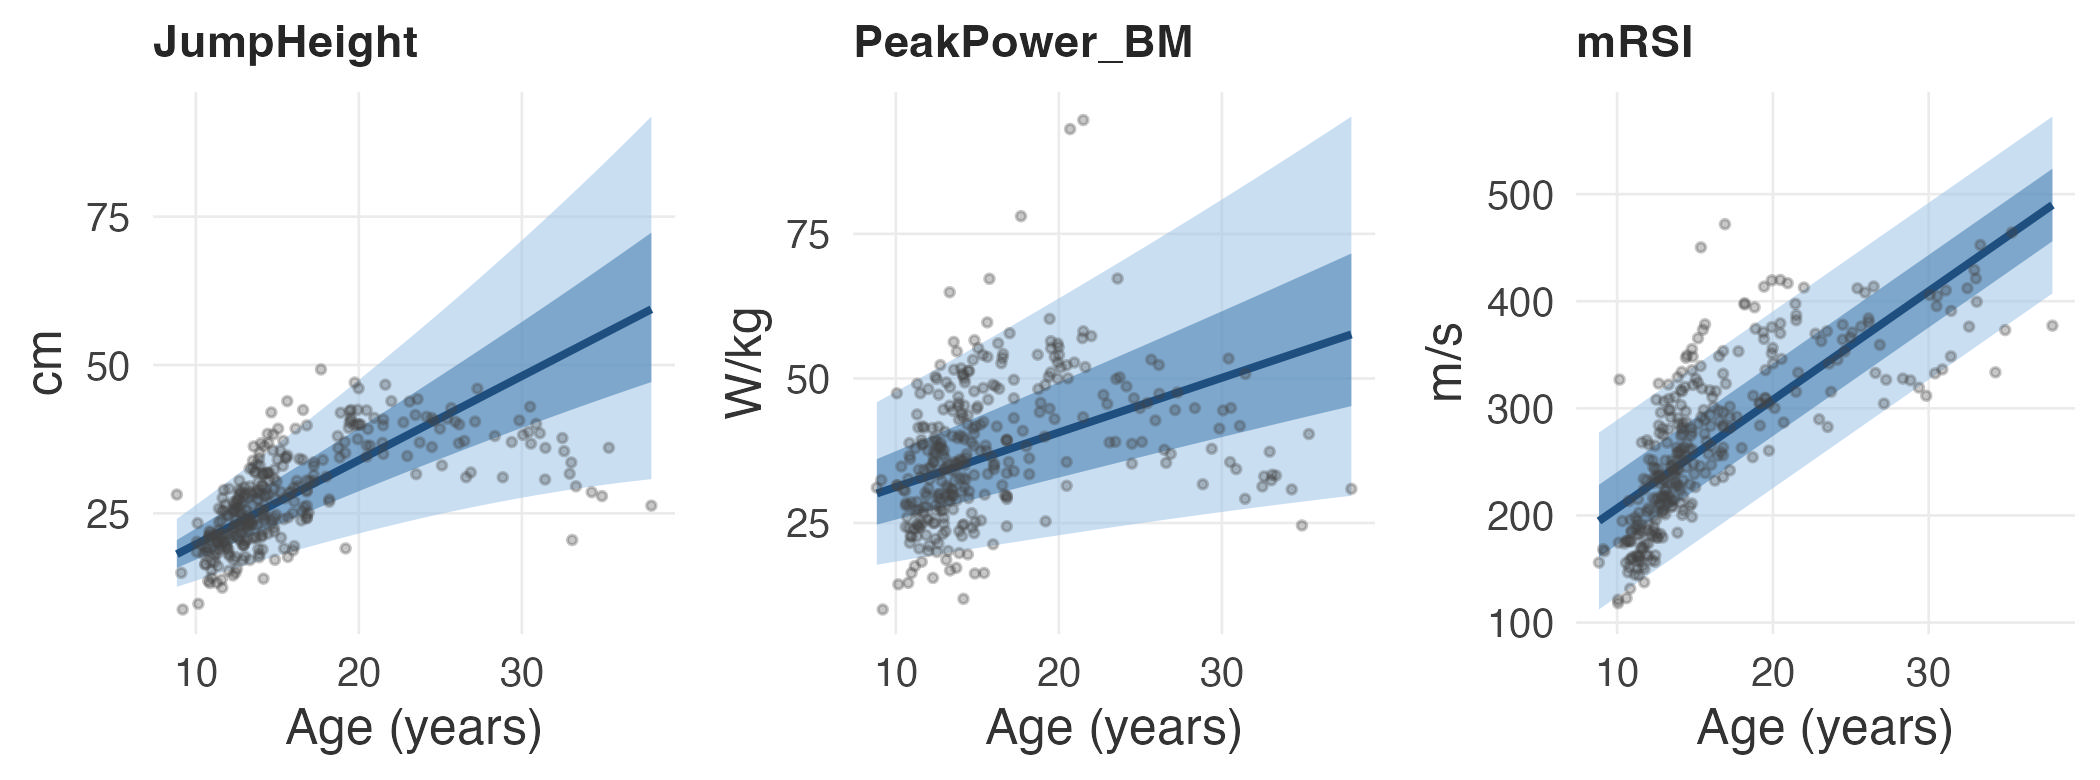
\includegraphics[width=\linewidth]{fig_centiles_example.jpg}
\end{minipage}\hfill
\begin{minipage}[c]{0.36\linewidth}\centering
  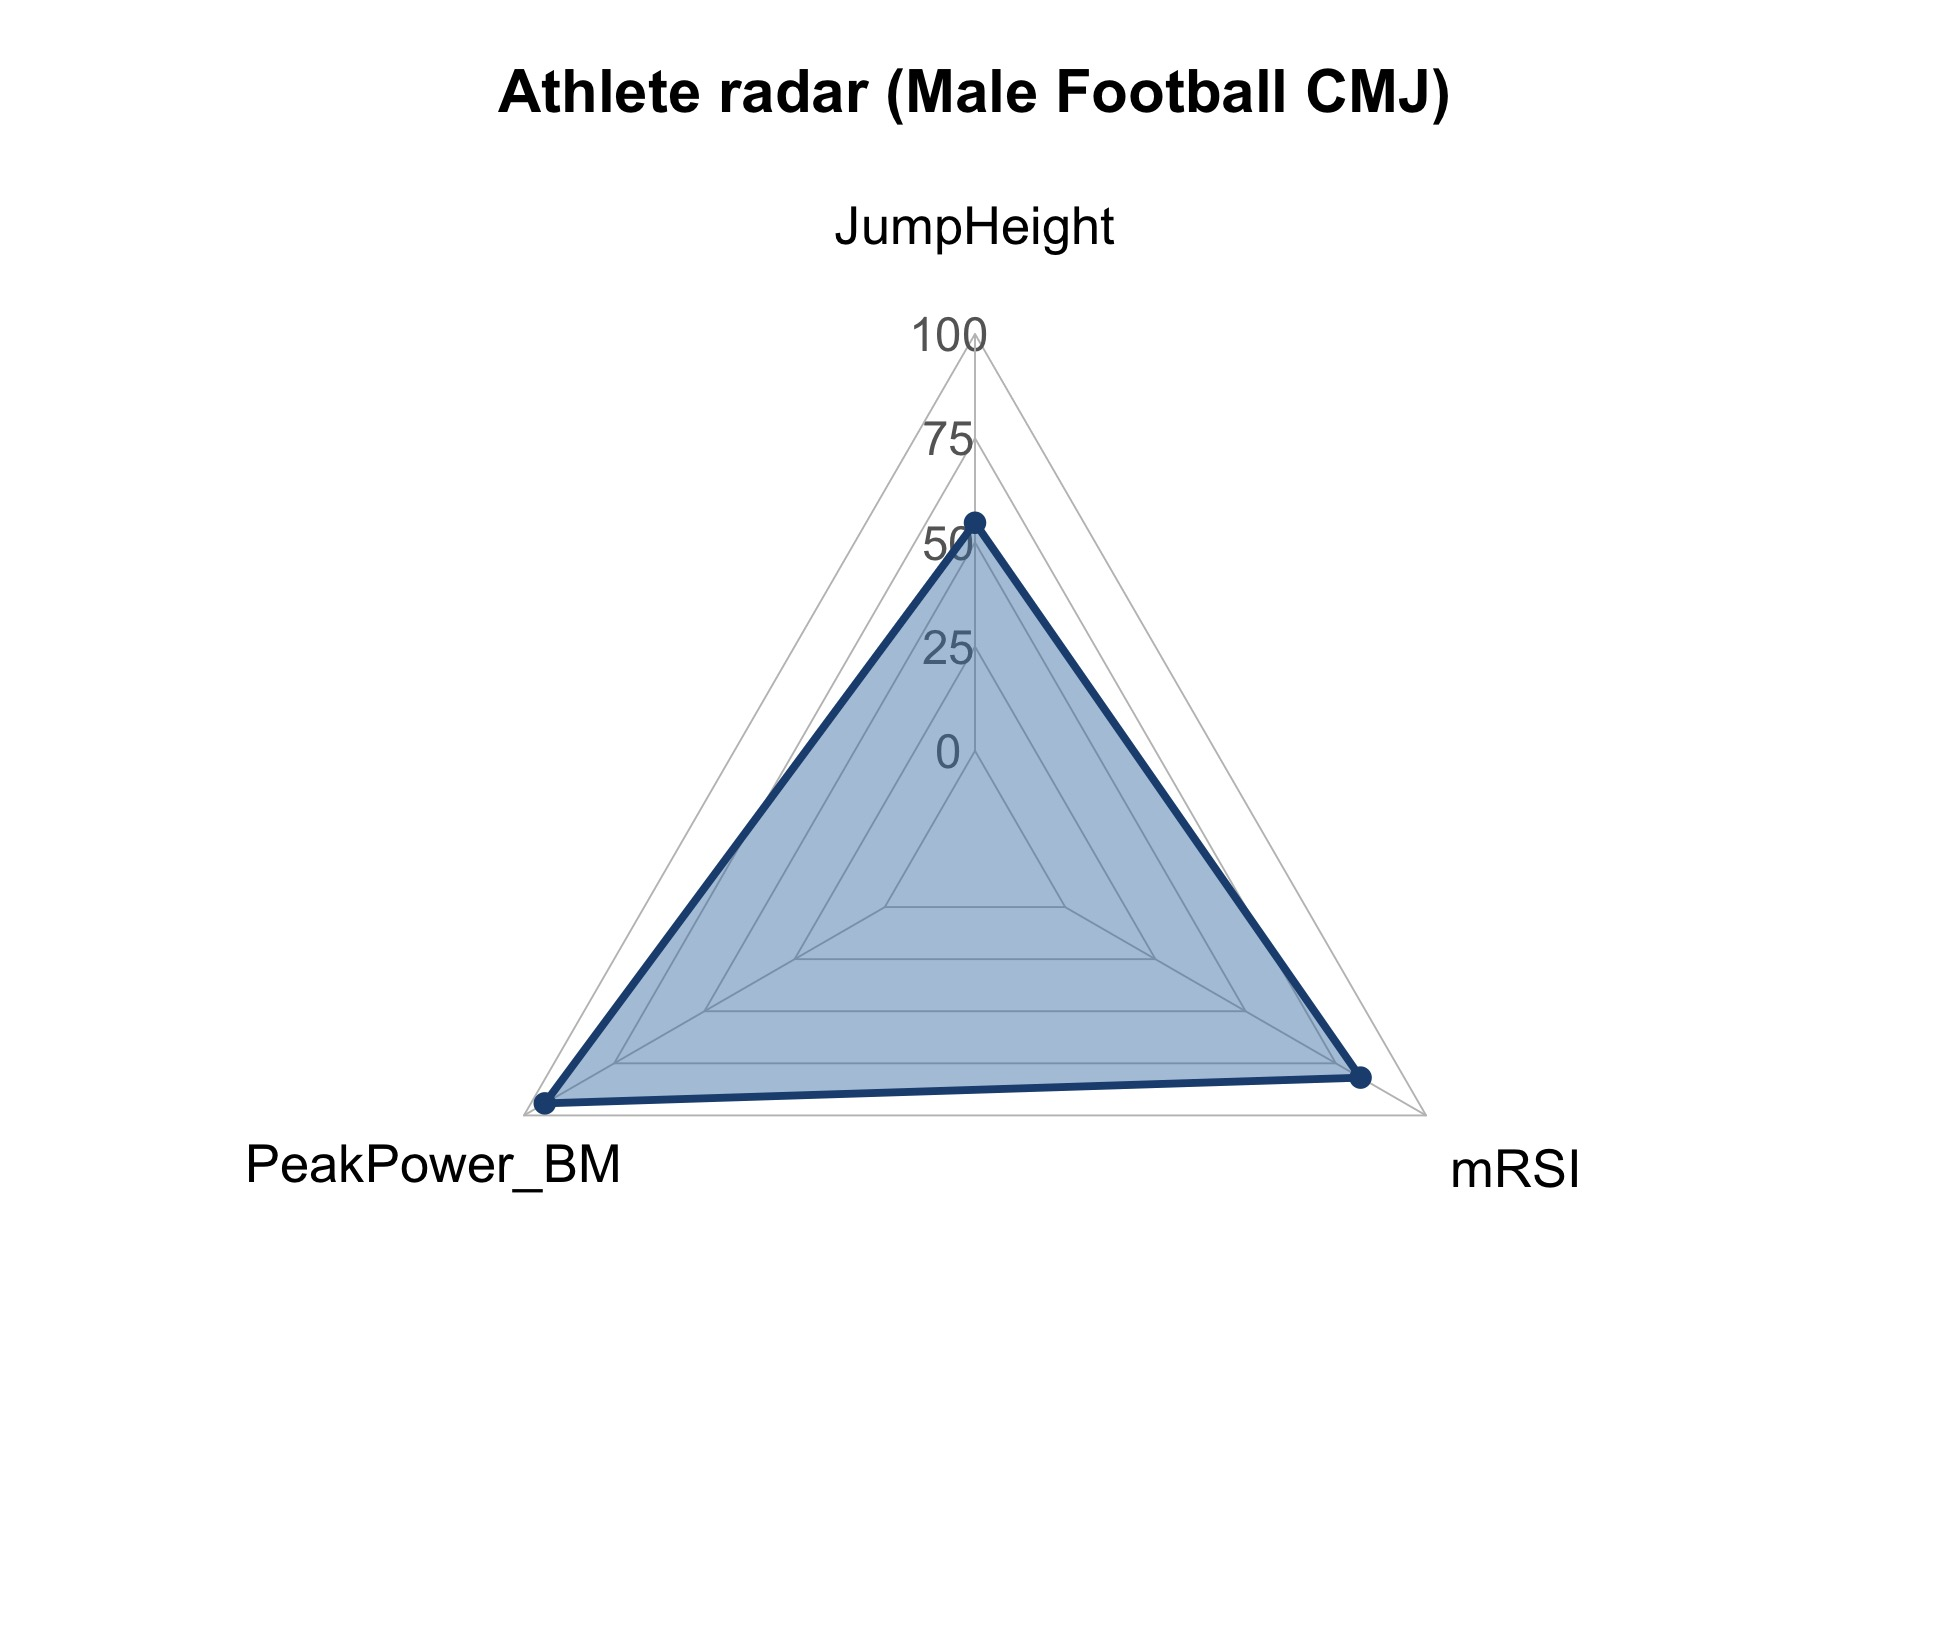
\includegraphics[width=\linewidth]{fig_radar_example.jpg}
\end{minipage}
\caption{Worked example. Left: per-metric age-conditional centile
bands (5/25/50/75/95) for Male Football CMJ; bands are model-based
predictive quantiles at the median body mass. Right: the same
athlete's per-metric percentiles on a $[0,100]$ axis. All three
marginal points sit above the cohort median, yet the joint pattern is
rare (Table~\ref{tab:score}).}
\label{fig:centiles}
\end{figure}

Centile bands for the same metric across all CMJ cohorts (so the
reader can compare the Male Football CMJ profile with other CMJ
cohorts) are in Appendix Figure~\ref{fig:centile_bands_grid}.

\FloatBarrier
\section{Discussion}
\label{sec:discussion}

\textbf{What we add.} The pipeline is, to our knowledge, the first
end-to-end implementation of multivariable centile profiling for
ForceDecks data that commits to a fixed clinical panel per protocol,
settles each cohort's marginal and joint structure through proper
scoring rules with cross-validation, and degrades gracefully under
low reliability or small sample sizes. The joint ES gain over
independence is modest in absolute terms (\MeanGain{}\,\% on average)
but always non-negative, and is largest in single-leg jump and drop
jump cohorts, where bilateral and stretch-shortening cycle dependence
is real biomechanics rather than measurement noise. For the
practitioner, the operational gain is the change in interpretation,
not the change in score: an athlete who looks elite under three
independent centile bands can sit in the bottom decile under the
joint model, and the worked example just above
(Sec.~\ref{sec:example}) is exactly that case.

\textbf{Where the pipeline binds.} Three constraints shape the
output: the reliability filter (the dominant one, matching the
ForceDecks profile reported by Cormack et al.\
\cite{cormack2008reliability} and Merrigan et al.\
\cite{merrigan2022forcedecks}), the sample-size cap
$n\!\geq\!10\binom{p}{2}$ that trims medium-sized cohorts to
$p\!=\!1$ or $p\!=\!2$, and uneven sport coverage:
\NsportsCohort{}~of \Nsports{}~sports yield a surviving cohort, and
football alone accounts for the majority of cohorts that support
$p\!\geq\!3$. None of these are pipeline failures; they are the cost
of refusing to fit a copula that the sample cannot identify.

\textbf{Limitations and future work.} We treat each test session
independently and do not model intra-athlete temporal dependence (an
athlete's repeated measurements through a season). The reliability
summary rests on a single test--retest design and assumes the
within-cohort population is homogeneous over the window in which the
retest pairs were collected. The fixed clinical panel is conservative
by design, so an athlete-specific candidate metric (e.g.\ a sport
coach's preferred asymmetry index) cannot enter the joint model
without re-running the per-cohort competition. Conditional vine
copulas~\cite{czado2022vinereview} that allow the dependence
structure itself to vary smoothly with age, body mass or playing
level are the natural next step, as is treating playing position as
a covariate where it is consistently recorded.

\section{Conclusion}
\label{sec:conclusion}

We provide a fully scripted, sex-stratified, reliability-aware
pipeline for multivariable centile modelling of ForceDecks data. Its
three model competitions --- marginal candidates, joint candidates,
and per-cohort dimensionality --- make every modelling choice
defensible by a single number. The accompanying
\texttt{score\_athlete()} function returns marginal percentiles with
measurement-noise context and a bootstrap-stabilised joint percentile,
surfacing the joint phenotypes that no per-metric report can detect.

\appendix
\renewcommand{\thesection}{\Alph{section}}

\section{Cohort coverage}
\label{app:coverage}
\noindent Sample size $n$ per sex\,$\times$\,sport\,$\times$\,test
cohort. Empty cells indicate cohorts that did not survive eligibility
($n < 25$). The best-covered cells are Male Football CMJ ($n = 333$),
Male Football DJ ($n = 328$) and Male Football SLJ ($n = 308$); the
thinnest are Male Badminton DJ ($n = 25$), Male Cricket SLLAH
($n = 25$) and Male Swimming SLJ ($n = 26$). Female cohorts and
non-football sports are systematically smaller, which is the source
of the variable-selection patterns reported in Sec.~\ref{sec:results}.

\smallskip
\begin{center}\scriptsize
\setlength{\tabcolsep}{3pt}
\begin{tabular}{lcccccccccccccc}
\toprule
Sport & \multicolumn{7}{c}{Male} & \multicolumn{7}{c}{Female} \\
\cmidrule(lr){2-8}\cmidrule(lr){9-15}
 & CMJ & DJ & SJ & SLJ & SLDJ & SLLAH & SLHAR & CMJ & DJ & SJ & SLJ & SLDJ & SLLAH & SLHAR \\
\midrule
Badminton & 85 & 25 &  &  &  &  &  & 37 & 33 &  &  &  &  & 30 \\
Basketball & 73 &  &  &  &  &  &  &  &  &  &  &  &  &  \\
Cricket & 46 & 31 &  &  &  & 25 &  &  &  &  &  &  &  &  \\
Football & 333 & 328 & 188 & 308 & 156 & 225 & 166 & 82 & 71 &  & 67 & 55 & 63 & 55 \\
Swimming & 27 &  &  & 26 &  &  &  &  &  &  &  &  &  &  \\
Track and Field & 29 &  &  &  &  &  &  &  &  &  &  &  &  &  \\
\bottomrule
\end{tabular}
\setlength{\tabcolsep}{6pt}

\end{center}
\refstepcounter{table}\label{tab:coverage}

\section{Additional EDA panels}
\label{app:eda}
\begin{center}
\begin{minipage}{0.24\linewidth}
  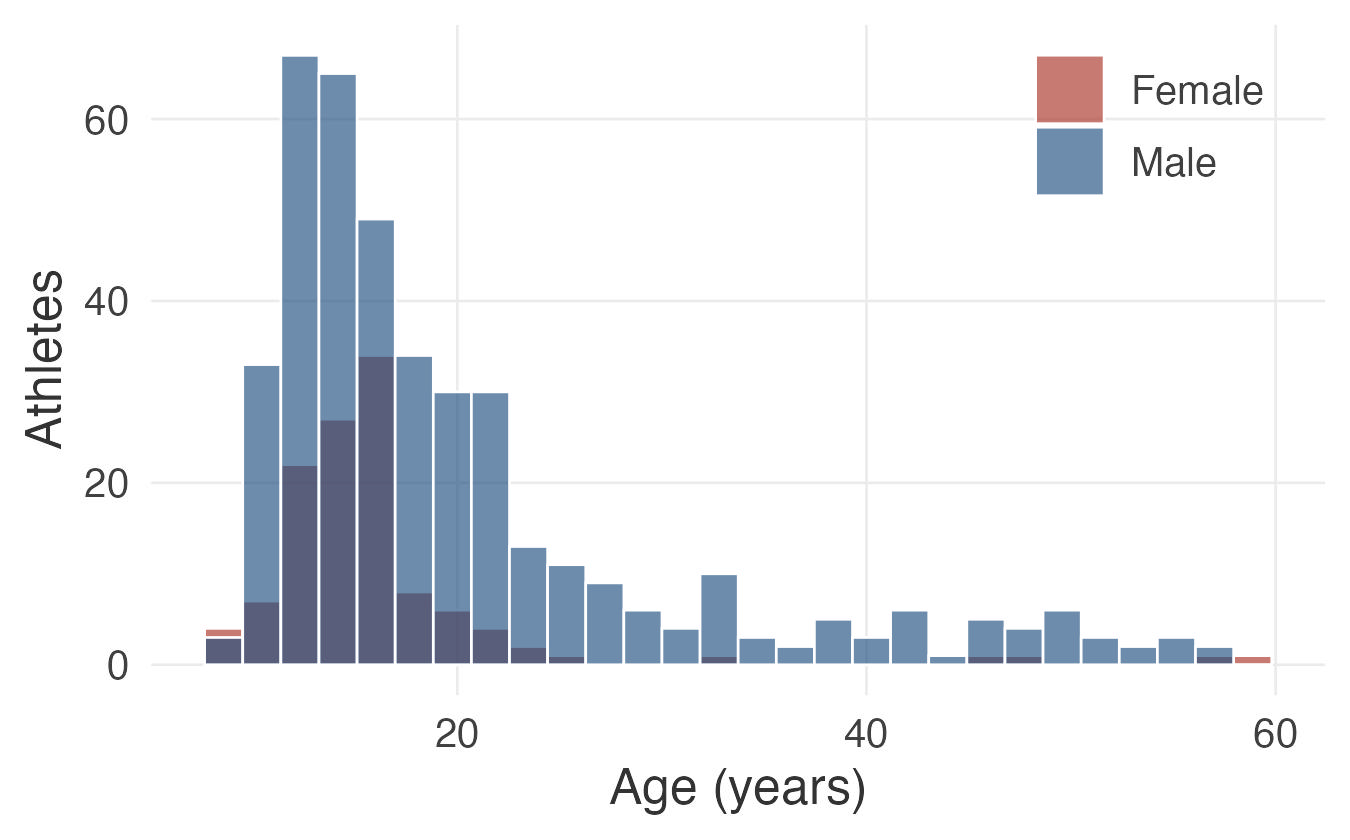
\includegraphics[width=\linewidth]{fig_eda_age.jpg}\\
  \captionof{figure}{Athlete age distribution.}
\end{minipage}\hfill
\begin{minipage}{0.24\linewidth}
  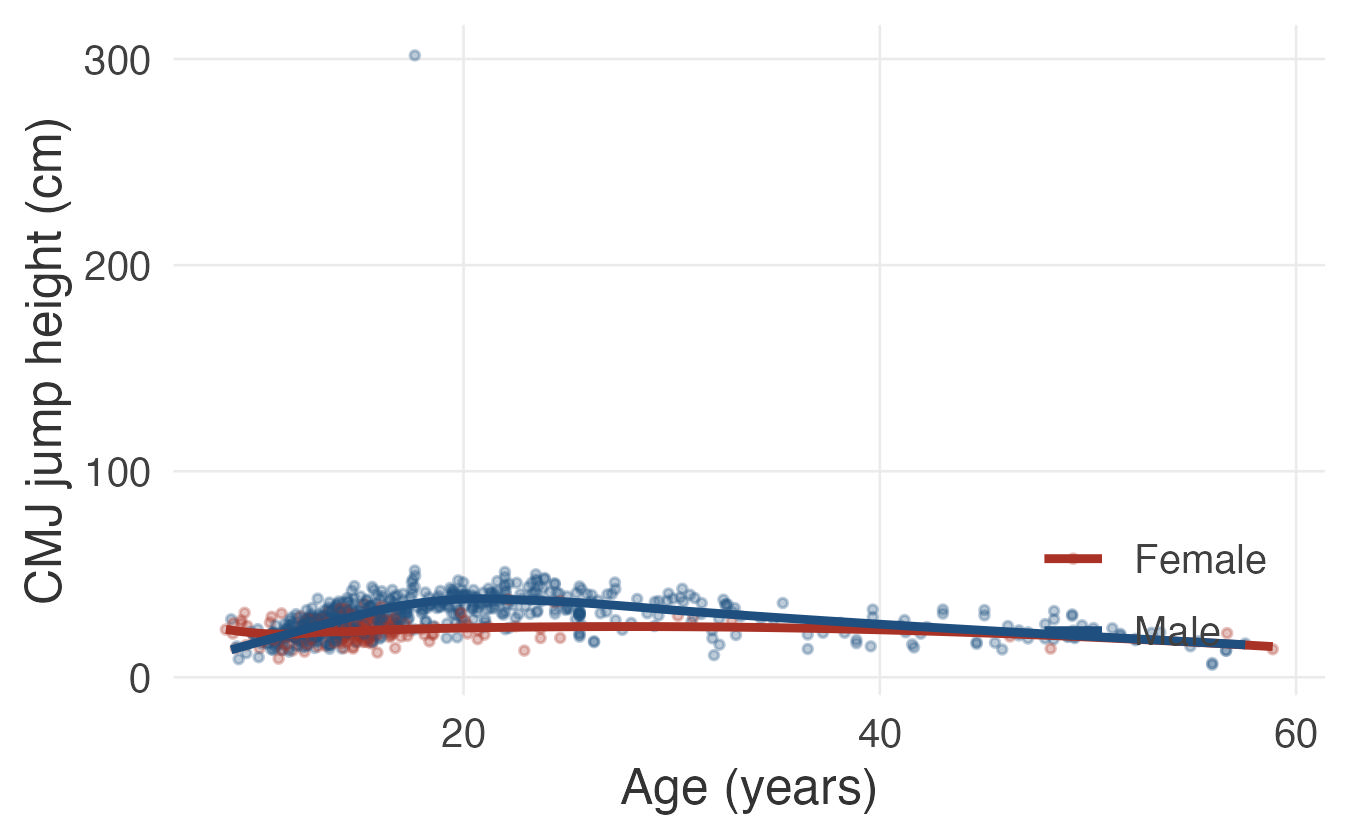
\includegraphics[width=\linewidth]{fig_eda_jh_age.jpg}\\
  \captionof{figure}{CMJ jump height vs.\ age by sex.}
\end{minipage}\hfill
\begin{minipage}{0.24\linewidth}
  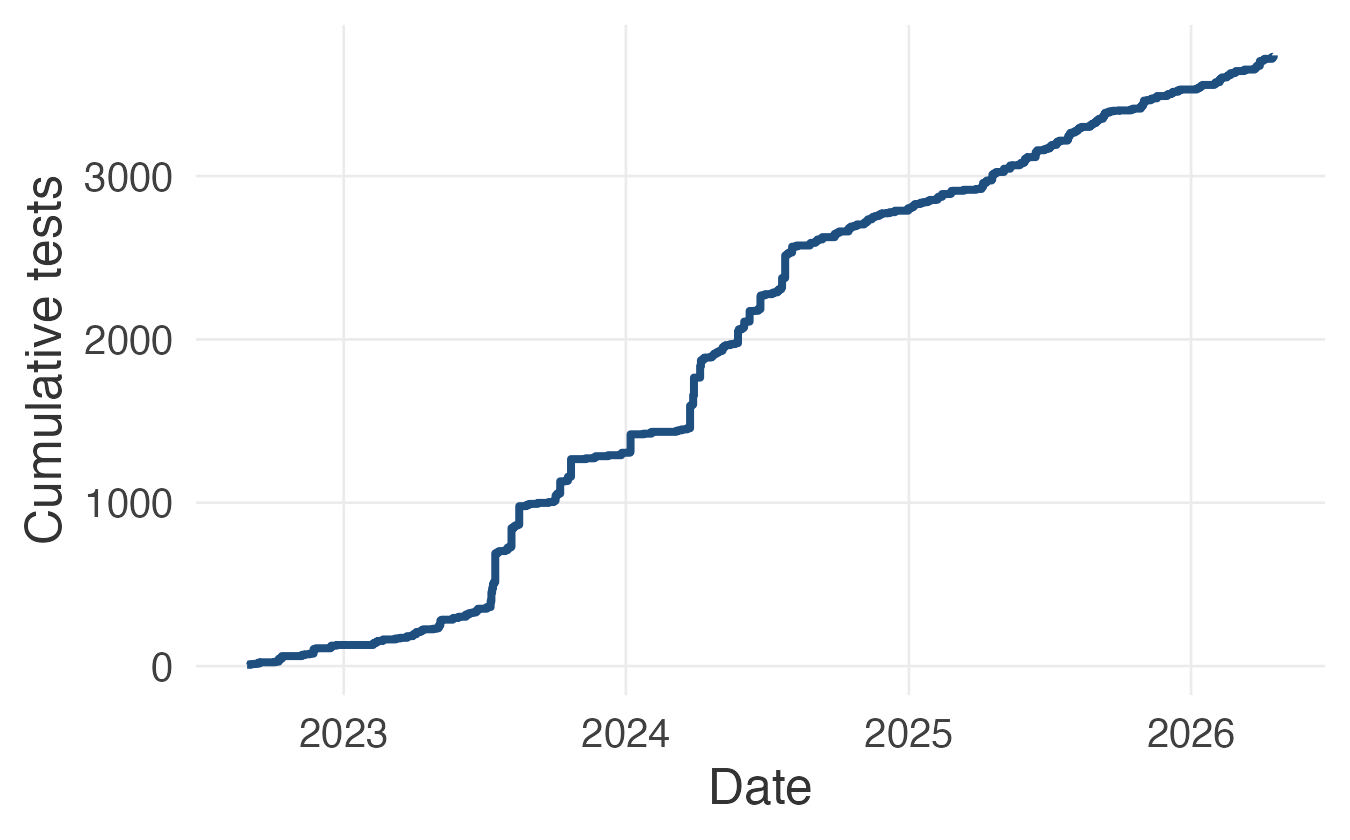
\includegraphics[width=\linewidth]{fig_eda_cumulative.jpg}\\
  \captionof{figure}{Cumulative tests over time.}
\end{minipage}\hfill
\begin{minipage}{0.24\linewidth}
  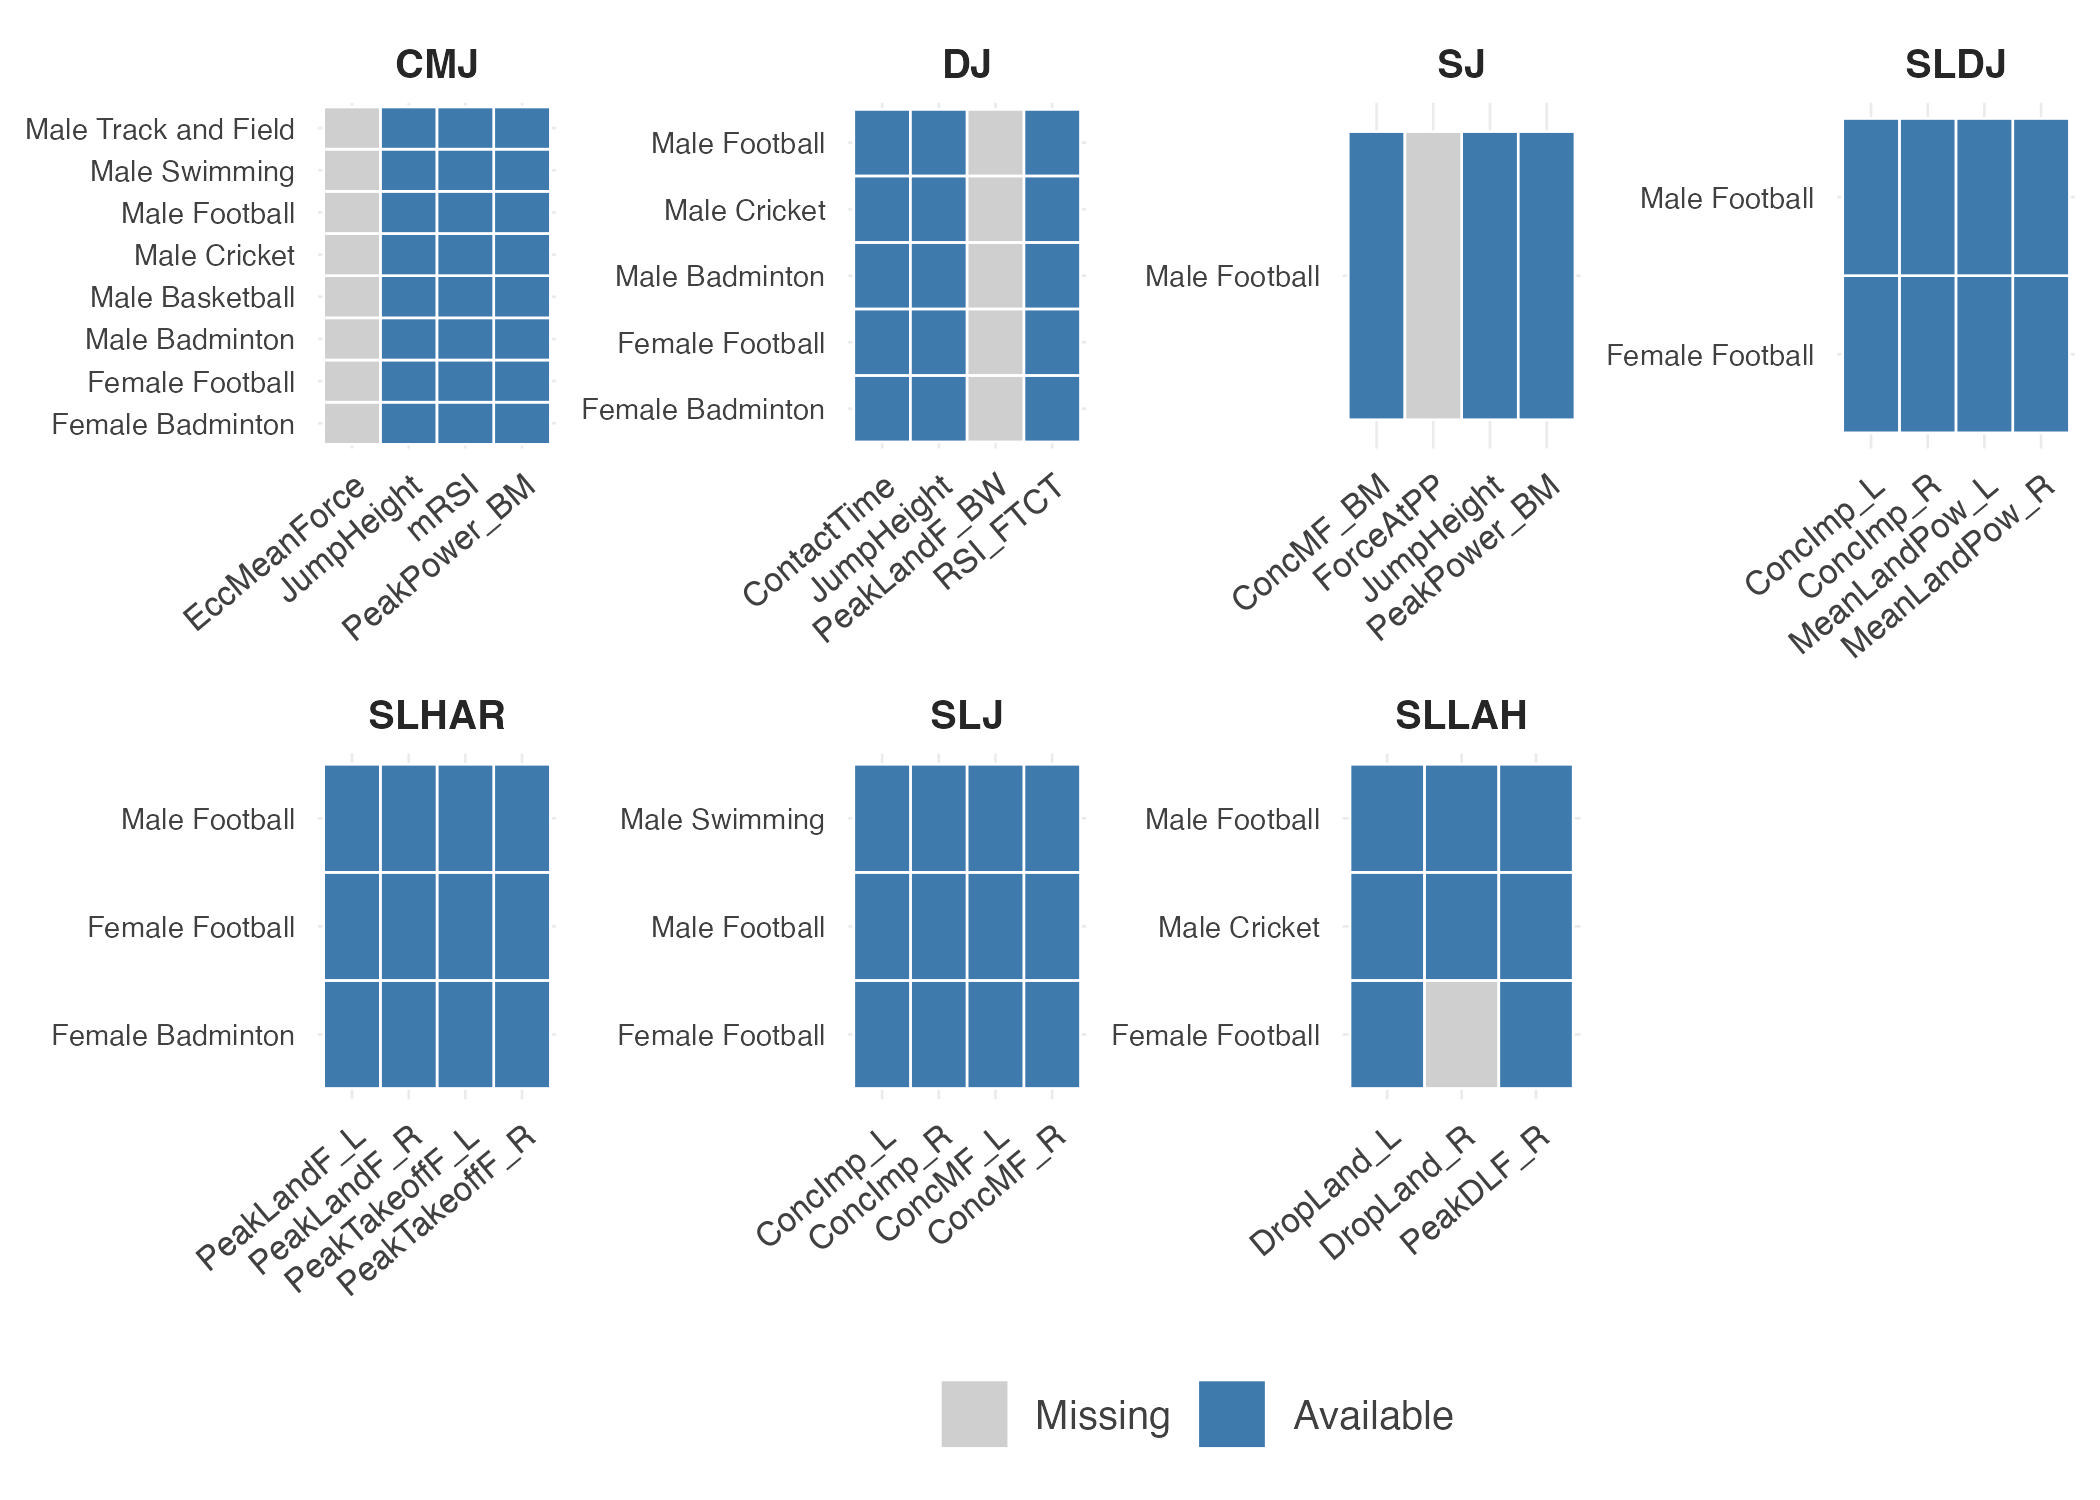
\includegraphics[width=\linewidth]{fig_eda_missing.jpg}\\
  \captionof{figure}{Panel availability per cohort.}
\end{minipage}
\end{center}

\section{Per-cohort reliability (full)}
\label{app:reliability_full}
The unaggregated Stage~2 output: every (sex, sport, test, metric) cell
that contributed to the body Table~\ref{tab:reliability} summary,
with its own ICC$_{(3,1)}$, SEM and MDC$_{95}$.
{\small
\begin{longtable}{lllrlrrr}
\caption{\textbf{Per-cohort reliability table (full):} every (sex, sport, test, metric) cell with its own ICC$_{(3,1)}$, SEM and MDC$_{95}$ from the test--retest pair construction in Methodology Stage~2.}\label{tab:reliability_full}\\
\toprule
Sex & Sport & Test & Metric & $n$ pairs & ICC$_{(3,1)}$ & SEM & MDC$_{95}$ \\
\midrule
\endfirsthead
\multicolumn{8}{l}{\emph{(continued)}} \\
\toprule
Sex & Sport & Test & Metric & $n$ pairs & ICC$_{(3,1)}$ & SEM & MDC$_{95}$ \\
\midrule
\endhead
\bottomrule
\endfoot
Female & Badminton & CMJ & \texttt{JumpHeight} & 6 & 0.38 & 4.83 & 13.40 \\
Female & Badminton & CMJ & \texttt{mRSI} & 6 & 0.98 & 5.99 & 16.60 \\
Female & Badminton & CMJ & \texttt{PeakPower\_BM} & 6 & 0.27 & 9.43 & 26.10 \\
Female & Football & CMJ & \texttt{JumpHeight} & 15 & 0.47 & 2.53 & 7.01 \\
Female & Football & CMJ & \texttt{mRSI} & 15 & 0.82 & 21.10 & 58.50 \\
Female & Football & CMJ & \texttt{PeakPower\_BM} & 15 & 0.25 & 6.67 & 18.50 \\
Male & Badminton & CMJ & \texttt{JumpHeight} & 8 & 0.80 & 3.51 & 9.73 \\
Male & Badminton & CMJ & \texttt{mRSI} & 8 & 0.96 & 11.50 & 31.90 \\
Male & Badminton & CMJ & \texttt{PeakPower\_BM} & 8 & 0.63 & 7.43 & 20.60 \\
Male & Basketball & CMJ & \texttt{JumpHeight} & 0 & NA & NA & NA \\
Male & Basketball & CMJ & \texttt{mRSI} & 0 & NA & NA & NA \\
Male & Basketball & CMJ & \texttt{PeakPower\_BM} & 0 & NA & NA & NA \\
Male & Cricket & CMJ & \texttt{JumpHeight} & 6 & 0.82 & 3.31 & 9.16 \\
Male & Cricket & CMJ & \texttt{mRSI} & 6 & 0.51 & 48.70 & 135.00 \\
Male & Cricket & CMJ & \texttt{PeakPower\_BM} & 6 & 0.66 & 7.40 & 20.50 \\
Male & Football & CMJ & \texttt{JumpHeight} & 80 & 0.88 & 2.83 & 7.84 \\
Male & Football & CMJ & \texttt{mRSI} & 80 & 0.97 & 11.70 & 32.40 \\
Male & Football & CMJ & \texttt{PeakPower\_BM} & 80 & 0.51 & 7.61 & 21.10 \\
Male & Swimming & CMJ & \texttt{JumpHeight} & 0 & NA & NA & NA \\
Male & Swimming & CMJ & \texttt{mRSI} & 0 & NA & NA & NA \\
Male & Swimming & CMJ & \texttt{PeakPower\_BM} & 0 & NA & NA & NA \\
Male & Track and Field & CMJ & \texttt{JumpHeight} & 0 & NA & NA & NA \\
Male & Track and Field & CMJ & \texttt{mRSI} & 0 & NA & NA & NA \\
Male & Track and Field & CMJ & \texttt{PeakPower\_BM} & 0 & NA & NA & NA \\
\addlinespace[1pt]
Female & Badminton & DJ & \texttt{ContactTime} & 0 & NA & NA & NA \\
Female & Badminton & DJ & \texttt{JumpHeight} & 0 & NA & NA & NA \\
Female & Badminton & DJ & \texttt{PeakLandF\_BW} & 0 & NA & NA & NA \\
Female & Badminton & DJ & \texttt{RSI\_FTCT} & 0 & NA & NA & NA \\
Female & Football & DJ & \texttt{ContactTime} & 17 & 0.81 & 0.05 & 0.13 \\
Female & Football & DJ & \texttt{JumpHeight} & 17 & 0.84 & 2.41 & 6.67 \\
Female & Football & DJ & \texttt{PeakLandF\_BW} & 0 & NA & NA & NA \\
Female & Football & DJ & \texttt{RSI\_FTCT} & 17 & 0.81 & 0.18 & 0.50 \\
Male & Badminton & DJ & \texttt{ContactTime} & 6 & 0.78 & 0.07 & 0.19 \\
Male & Badminton & DJ & \texttt{JumpHeight} & 6 & 0.63 & 4.50 & 12.50 \\
Male & Badminton & DJ & \texttt{PeakLandF\_BW} & 0 & NA & NA & NA \\
Male & Badminton & DJ & \texttt{RSI\_FTCT} & 6 & 0.82 & 0.22 & 0.61 \\
Male & Cricket & DJ & \texttt{ContactTime} & 0 & NA & NA & NA \\
Male & Cricket & DJ & \texttt{JumpHeight} & 0 & NA & NA & NA \\
Male & Cricket & DJ & \texttt{PeakLandF\_BW} & 0 & NA & NA & NA \\
Male & Cricket & DJ & \texttt{RSI\_FTCT} & 0 & NA & NA & NA \\
Male & Football & DJ & \texttt{ContactTime} & 84 & 0.39 & 0.10 & 0.27 \\
Male & Football & DJ & \texttt{JumpHeight} & 84 & 0.83 & 3.57 & 9.90 \\
Male & Football & DJ & \texttt{PeakLandF\_BW} & 0 & NA & NA & NA \\
Male & Football & DJ & \texttt{RSI\_FTCT} & 84 & 0.53 & 0.37 & 1.03 \\
\addlinespace[1pt]
Male & Football & SJ & \texttt{ConcMF\_BM} & 43 & 0.93 & 31.50 & 87.40 \\
Male & Football & SJ & \texttt{JumpHeight} & 43 & 0.00 & 1320.00 & 3650.00 \\
Male & Football & SJ & \texttt{PeakPower\_BM} & 43 & 0.27 & 0.98 & 2.71 \\
\addlinespace[1pt]
Female & Football & SLDJ & \texttt{ConcImp\_L} & 15 & 0.00 & 16.80 & 46.70 \\
Female & Football & SLDJ & \texttt{ConcImp\_R} & 15 & 0.02 & 18.30 & 50.80 \\
Female & Football & SLDJ & \texttt{MeanLandPow\_L} & 15 & 0.35 & 132.00 & 366.00 \\
Female & Football & SLDJ & \texttt{MeanLandPow\_R} & 15 & 0.57 & 130.00 & 359.00 \\
Male & Football & SLDJ & \texttt{ConcImp\_L} & 35 & 0.94 & 10.30 & 28.50 \\
Male & Football & SLDJ & \texttt{ConcImp\_R} & 35 & 0.93 & 11.20 & 31.20 \\
Male & Football & SLDJ & \texttt{MeanLandPow\_L} & 35 & 0.71 & 166.00 & 460.00 \\
Male & Football & SLDJ & \texttt{MeanLandPow\_R} & 35 & 0.74 & 148.00 & 410.00 \\
\addlinespace[1pt]
Female & Badminton & SLHAR & \texttt{PeakLandF\_L} & 0 & NA & NA & NA \\
Female & Badminton & SLHAR & \texttt{PeakLandF\_R} & 0 & NA & NA & NA \\
Female & Badminton & SLHAR & \texttt{PeakTakeoffF\_L} & 0 & NA & NA & NA \\
Female & Badminton & SLHAR & \texttt{PeakTakeoffF\_R} & 0 & NA & NA & NA \\
Female & Football & SLHAR & \texttt{PeakLandF\_L} & 15 & 0.69 & 196.00 & 544.00 \\
Female & Football & SLHAR & \texttt{PeakLandF\_R} & 15 & 0.78 & 177.00 & 491.00 \\
Female & Football & SLHAR & \texttt{PeakTakeoffF\_L} & 15 & 0.67 & 126.00 & 349.00 \\
Female & Football & SLHAR & \texttt{PeakTakeoffF\_R} & 15 & 0.71 & 120.00 & 333.00 \\
Male & Football & SLHAR & \texttt{PeakLandF\_L} & 35 & 0.90 & 189.00 & 523.00 \\
Male & Football & SLHAR & \texttt{PeakLandF\_R} & 35 & 0.89 & 184.00 & 509.00 \\
Male & Football & SLHAR & \texttt{PeakTakeoffF\_L} & 35 & 0.90 & 154.00 & 428.00 \\
Male & Football & SLHAR & \texttt{PeakTakeoffF\_R} & 35 & 0.91 & 157.00 & 435.00 \\
\addlinespace[1pt]
Female & Football & SLJ & \texttt{ConcImp\_L} & 15 & 0.18 & 15.10 & 41.80 \\
Female & Football & SLJ & \texttt{ConcImp\_R} & 15 & 0.63 & 7.25 & 20.10 \\
Female & Football & SLJ & \texttt{ConcMF\_L} & 15 & 0.54 & 110.00 & 306.00 \\
Female & Football & SLJ & \texttt{ConcMF\_R} & 15 & 0.92 & 41.40 & 115.00 \\
Male & Football & SLJ & \texttt{ConcImp\_L} & 79 & 0.89 & 11.80 & 32.80 \\
Male & Football & SLJ & \texttt{ConcImp\_R} & 81 & 0.88 & 13.20 & 36.50 \\
Male & Football & SLJ & \texttt{ConcMF\_L} & 79 & 0.89 & 81.90 & 227.00 \\
Male & Football & SLJ & \texttt{ConcMF\_R} & 81 & 0.84 & 98.00 & 272.00 \\
Male & Swimming & SLJ & \texttt{ConcImp\_L} & 0 & NA & NA & NA \\
Male & Swimming & SLJ & \texttt{ConcImp\_R} & 0 & NA & NA & NA \\
Male & Swimming & SLJ & \texttt{ConcMF\_L} & 0 & NA & NA & NA \\
Male & Swimming & SLJ & \texttt{ConcMF\_R} & 0 & NA & NA & NA \\
\addlinespace[1pt]
Female & Football & SLLAH & \texttt{DropLand\_L} & 14 & 0.00 & 106.00 & 293.00 \\
Female & Football & SLLAH & \texttt{DropLand\_R} & 14 & 0.00 & 104.00 & 287.00 \\
Female & Football & SLLAH & \texttt{PeakDLF\_R} & 14 & 0.59 & 272.00 & 754.00 \\
Male & Cricket & SLLAH & \texttt{DropLand\_L} & 0 & NA & NA & NA \\
Male & Cricket & SLLAH & \texttt{DropLand\_R} & 0 & NA & NA & NA \\
Male & Cricket & SLLAH & \texttt{PeakDLF\_R} & 0 & NA & NA & NA \\
Male & Football & SLLAH & \texttt{DropLand\_L} & 45 & 0.00 & 119.00 & 329.00 \\
Male & Football & SLLAH & \texttt{DropLand\_R} & 45 & 0.00 & 108.00 & 298.00 \\
Male & Football & SLLAH & \texttt{PeakDLF\_R} & 45 & 0.49 & 442.00 & 1220.00 \\
\end{longtable}
}


\section{Per-cohort marginal-competition (full)}
\label{app:marg_full}
The full per-(cohort $\times$ metric) Stage~4 marginal competition
under Eq.~\eqref{eq:crps}: 5-fold cross-validated CRPS$/$IQR for
Linear (M1, Eq.~\eqref{eq:m1}), GAMLSS-NO (M2, Eq.~\eqref{eq:m2}) and
GAMLSS-BCT (M3, Eq.~\eqref{eq:m3}). The winning family is bolded.
{\small
\begin{longtable}{lllllrrrl}
\caption{\textbf{Per-(cohort $\times$ metric) marginal-competition (full):} 5-fold cross-validated CRPS$/$IQR (lower is sharper) for the three candidate marginals defined in Eqs.~(1)--(3); \textbf{bold} = winner under Eq.~(4).}\label{tab:marg_full}\\
\toprule
Sex & Sport & Test & Metric & MassDep & Linear & NO & BCT & Winner \\
\midrule
\endfirsthead
\multicolumn{9}{l}{\emph{(continued)}} \\
\toprule
Sex & Sport & Test & Metric & MassDep & Linear & NO & BCT & Winner \\
\midrule
\endhead
\bottomrule
\endfoot
Female & Badminton & CMJ & \texttt{JumpHeight} & no & \textbf{0.417} & 0.432 & 0.424 & Linear \\
Female & Badminton & CMJ & \texttt{mRSI} & no & 0.385 & 0.405 & \textbf{0.379} & BCT \\
Female & Badminton & CMJ & \texttt{PeakPower\_BM} & no & \textbf{0.506} & 0.521 & 0.511 & Linear \\
Female & Football & CMJ & \texttt{JumpHeight} & no & 0.505 & 0.505 & \textbf{0.498} & BCT \\
Female & Football & CMJ & \texttt{mRSI} & no & \textbf{0.466} & 0.477 & 0.475 & Linear \\
Female & Football & CMJ & \texttt{PeakPower\_BM} & no & 0.399 & 0.402 & \textbf{0.399} & BCT \\
Male & Badminton & CMJ & \texttt{JumpHeight} & no & 0.342 & \textbf{0.335} & 0.337 & NO \\
Male & Badminton & CMJ & \texttt{mRSI} & no & \textbf{0.452} & 0.464 & 0.454 & Linear \\
Male & Badminton & CMJ & \texttt{PeakPower\_BM} & no & 0.359 & 0.364 & \textbf{0.332} & BCT \\
Male & Basketball & CMJ & \texttt{JumpHeight} & no & 0.400 & 0.401 & \textbf{0.396} & BCT \\
Male & Basketball & CMJ & \texttt{mRSI} & no & 0.467 & \textbf{0.458} & 0.459 & NO \\
Male & Basketball & CMJ & \texttt{PeakPower\_BM} & no & 0.477 & 0.477 & \textbf{0.475} & BCT \\
Male & Cricket & CMJ & \texttt{JumpHeight} & no & \textbf{0.475} & 0.515 & 0.487 & Linear \\
Male & Cricket & CMJ & \texttt{mRSI} & no & 0.448 & 0.466 & \textbf{0.441} & BCT \\
Male & Cricket & CMJ & \texttt{PeakPower\_BM} & no & \textbf{0.437} & 0.457 & 0.471 & Linear \\
Male & Football & CMJ & \texttt{JumpHeight} & no & 0.283 & 0.283 & \textbf{0.280} & BCT \\
Male & Football & CMJ & \texttt{mRSI} & no & \textbf{0.247} & 0.251 & 0.257 & Linear \\
Male & Football & CMJ & \texttt{PeakPower\_BM} & no & 0.406 & 0.411 & \textbf{0.406} & BCT \\
Male & Swimming & CMJ & \texttt{JumpHeight} & no & \textbf{0.333} & 0.348 & 0.361 & Linear \\
Male & Swimming & CMJ & \texttt{mRSI} & no & \textbf{0.462} & 0.478 & 0.491 & Linear \\
Male & Swimming & CMJ & \texttt{PeakPower\_BM} & no & \textbf{0.387} & 0.397 & 0.401 & Linear \\
Male & Track and Field & CMJ & \texttt{JumpHeight} & no & 0.276 & 0.922 & \textbf{0.250} & BCT \\
Male & Track and Field & CMJ & \texttt{mRSI} & no & \textbf{0.435} & 0.656 & 0.463 & Linear \\
Male & Track and Field & CMJ & \texttt{PeakPower\_BM} & no & \textbf{0.375} & 0.617 & 0.388 & Linear \\
\addlinespace[1pt]
Female & Badminton & DJ & \texttt{ContactTime} & no & 0.363 & 0.358 & \textbf{0.353} & BCT \\
Female & Badminton & DJ & \texttt{JumpHeight} & no & 0.359 & 0.368 & \textbf{0.357} & BCT \\
Female & Badminton & DJ & \texttt{RSI\_FTCT} & no & 0.479 & 0.505 & \textbf{0.446} & BCT \\
Female & Football & DJ & \texttt{ContactTime} & no & \textbf{0.455} & 0.457 & 0.463 & Linear \\
Female & Football & DJ & \texttt{JumpHeight} & no & 0.489 & 0.481 & \textbf{0.452} & BCT \\
Female & Football & DJ & \texttt{RSI\_FTCT} & no & 0.401 & 0.409 & \textbf{0.396} & BCT \\
Male & Badminton & DJ & \texttt{ContactTime} & no & \textbf{0.408} & 0.410 & 0.421 & Linear \\
Male & Badminton & DJ & \texttt{JumpHeight} & no & 0.373 & \textbf{0.366} & 0.374 & NO \\
Male & Badminton & DJ & \texttt{RSI\_FTCT} & no & 0.418 & 0.423 & \textbf{0.412} & BCT \\
Male & Cricket & DJ & \texttt{ContactTime} & no & \textbf{0.446} & 0.474 & 0.504 & Linear \\
Male & Cricket & DJ & \texttt{JumpHeight} & no & 0.480 & 0.413 & \textbf{0.371} & BCT \\
Male & Cricket & DJ & \texttt{RSI\_FTCT} & no & \textbf{0.381} & 0.413 & 0.421 & Linear \\
Male & Football & DJ & \texttt{ContactTime} & no & \textbf{0.386} & 0.391 & 0.387 & Linear \\
Male & Football & DJ & \texttt{JumpHeight} & no & \textbf{0.297} & 0.300 & 0.298 & Linear \\
Male & Football & DJ & \texttt{RSI\_FTCT} & no & 0.414 & 0.416 & \textbf{0.413} & BCT \\
\addlinespace[1pt]
Male & Football & SJ & \texttt{ConcMF\_BM} & no & 0.253 & \textbf{0.237} & 0.238 & NO \\
Male & Football & SJ & \texttt{JumpHeight} & no & 0.158 & 0.455 & \textbf{0.121} & BCT \\
Male & Football & SJ & \texttt{PeakPower\_BM} & no & 0.418 & \textbf{0.417} & 0.418 & NO \\
\addlinespace[1pt]
Female & Football & SLDJ & \texttt{ConcImp\_L} & yes & 0.443 & 0.444 & \textbf{0.414} & BCT \\
Female & Football & SLDJ & \texttt{ConcImp\_R} & yes & 0.481 & 0.513 & \textbf{0.431} & BCT \\
Female & Football & SLDJ & \texttt{MeanLandPow\_L} & yes & \textbf{0.378} & 0.560 & 0.389 & Linear \\
Female & Football & SLDJ & \texttt{MeanLandPow\_R} & yes & 0.392 & 0.537 & \textbf{0.374} & BCT \\
Male & Football & SLDJ & \texttt{ConcImp\_L} & yes & \textbf{0.166} & 0.225 & 0.171 & Linear \\
Male & Football & SLDJ & \texttt{ConcImp\_R} & yes & \textbf{0.162} & 0.220 & 0.183 & Linear \\
Male & Football & SLDJ & \texttt{MeanLandPow\_L} & yes & \textbf{0.309} & 0.329 & 0.309 & Linear \\
Male & Football & SLDJ & \texttt{MeanLandPow\_R} & yes & \textbf{0.243} & 0.273 & 0.256 & Linear \\
\addlinespace[1pt]
Female & Badminton & SLHAR & \texttt{PeakLandF\_L} & yes & \textbf{0.328} & 0.424 & 0.394 & Linear \\
Female & Badminton & SLHAR & \texttt{PeakLandF\_R} & yes & \textbf{0.428} & 0.563 & 0.500 & Linear \\
Female & Badminton & SLHAR & \texttt{PeakTakeoffF\_L} & yes & \textbf{0.385} & 0.713 & 0.411 & Linear \\
Female & Badminton & SLHAR & \texttt{PeakTakeoffF\_R} & yes & \textbf{0.387} & 0.550 & 0.398 & Linear \\
Female & Football & SLHAR & \texttt{PeakLandF\_L} & yes & \textbf{0.337} & 0.562 & 0.381 & Linear \\
Female & Football & SLHAR & \texttt{PeakLandF\_R} & yes & \textbf{0.224} & 0.546 & 0.242 & Linear \\
Female & Football & SLHAR & \texttt{PeakTakeoffF\_L} & yes & \textbf{0.263} & 0.515 & 0.322 & Linear \\
Female & Football & SLHAR & \texttt{PeakTakeoffF\_R} & yes & \textbf{0.192} & 0.439 & 0.195 & Linear \\
Male & Football & SLHAR & \texttt{PeakLandF\_L} & yes & \textbf{0.167} & 0.217 & 0.185 & Linear \\
Male & Football & SLHAR & \texttt{PeakLandF\_R} & yes & \textbf{0.165} & 0.225 & 0.165 & Linear \\
Male & Football & SLHAR & \texttt{PeakTakeoffF\_L} & yes & \textbf{0.162} & 0.203 & 0.175 & Linear \\
Male & Football & SLHAR & \texttt{PeakTakeoffF\_R} & yes & \textbf{0.151} & 0.221 & 0.159 & Linear \\
\addlinespace[1pt]
Female & Football & SLJ & \texttt{ConcImp\_L} & yes & \textbf{0.354} & 0.433 & 0.372 & Linear \\
Female & Football & SLJ & \texttt{ConcImp\_R} & yes & \textbf{0.366} & 0.479 & 0.427 & Linear \\
Female & Football & SLJ & \texttt{ConcMF\_L} & yes & 0.328 & 0.524 & \textbf{0.321} & BCT \\
Female & Football & SLJ & \texttt{ConcMF\_R} & yes & 0.341 & 0.545 & \textbf{0.297} & BCT \\
Male & Football & SLJ & \texttt{ConcImp\_L} & yes & \textbf{0.186} & 0.248 & 0.193 & Linear \\
Male & Football & SLJ & \texttt{ConcImp\_R} & yes & \textbf{0.181} & 0.247 & 0.186 & Linear \\
Male & Football & SLJ & \texttt{ConcMF\_L} & yes & 0.163 & 0.255 & \textbf{0.156} & BCT \\
Male & Football & SLJ & \texttt{ConcMF\_R} & yes & 0.163 & 0.274 & \textbf{0.158} & BCT \\
Male & Swimming & SLJ & \texttt{ConcImp\_L} & yes & 0.400 & \textbf{0.321} & 0.429 & NO \\
Male & Swimming & SLJ & \texttt{ConcImp\_R} & yes & 0.434 & \textbf{0.416} & 0.440 & NO \\
Male & Swimming & SLJ & \texttt{ConcMF\_L} & yes & 0.459 & \textbf{0.397} & 0.504 & NO \\
Male & Swimming & SLJ & \texttt{ConcMF\_R} & yes & \textbf{0.386} & 0.391 & 0.656 & Linear \\
\addlinespace[1pt]
Female & Football & SLLAH & \texttt{DropLand\_L} & yes & 0.416 & 0.417 & \textbf{0.388} & BCT \\
Female & Football & SLLAH & \texttt{DropLand\_R} & yes & 0.372 & 0.376 & \textbf{0.370} & BCT \\
Female & Football & SLLAH & \texttt{PeakDLF\_R} & yes & 0.361 & 0.411 & \textbf{0.355} & BCT \\
Male & Cricket & SLLAH & \texttt{DropLand\_L} & yes & 0.563 & \textbf{0.515} & 2.850 & NO \\
Male & Cricket & SLLAH & \texttt{DropLand\_R} & yes & 0.492 & \textbf{0.459} & 0.478 & NO \\
Male & Cricket & SLLAH & \texttt{PeakDLF\_R} & yes & \textbf{0.334} & 0.389 & 0.385 & Linear \\
Male & Football & SLLAH & \texttt{DropLand\_L} & yes & \textbf{0.381} & 0.388 & 0.390 & Linear \\
Male & Football & SLLAH & \texttt{DropLand\_R} & yes & \textbf{0.344} & 0.355 & 0.358 & Linear \\
Male & Football & SLLAH & \texttt{PeakDLF\_R} & yes & 0.364 & 0.375 & \textbf{0.364} & BCT \\
\end{longtable}
}


\section{Per-cohort joint-copula competition and fitted vine structures}
\label{app:joint_full}
The Stage~5 joint competition: per-cohort 5-fold cross-validated
multivariate Energy Score for Independence, Gaussian copula, and the
R-vine of Eq.~\eqref{eq:vine}. The winning candidate is bolded; the
``Gain'' column reports the per-cent improvement of the winner over
the Independence baseline.
{\small
\begin{longtable}{lllrrrrrlr}
\caption{\textbf{Per-cohort joint-copula competition (full):} 5-fold cross-validated multivariate Energy Score for Independence, Gaussian copula and the regular vine of Eq.~(6); \textbf{bold} = winner; ``Gain'' is the per-cent improvement of the winner over the Independence baseline.}\label{tab:joint_full}\\
\toprule
Sex & Sport & Test & $n$ & $p$ & ES Indep & ES Gaussian & ES Vine & Winner & Gain (\%) \\
\midrule
\endfirsthead
\multicolumn{10}{l}{\emph{(continued)}} \\
\toprule
Sex & Sport & Test & $n$ & $p$ & ES Indep & ES Gaussian & ES Vine & Winner & Gain (\%) \\
\midrule
\endhead
\bottomrule
\endfoot
Male & Badminton & CMJ & 85 & 3 & 0.318 & \textbf{0.313} & 0.314 & Gaussian & 1.3 \\
Male & Basketball & CMJ & 73 & 3 & 0.336 & 0.333 & \textbf{0.331} & Vine & 1.5 \\
Male & Cricket & CMJ & 46 & 3 & 0.330 & 0.327 & \textbf{0.327} & Vine & 1.0 \\
Male & Football & CMJ & 333 & 3 & 0.333 & 0.326 & \textbf{0.325} & Vine & 2.3 \\
Male & Swimming & CMJ & 27 & 2 & 0.260 & 0.261 & \textbf{0.253} & Vine & 2.8 \\
Male & Track and Field & CMJ & 29 & 2 & \textbf{0.240} & 0.247 & 0.249 & Indep & 0.0 \\
Female & Badminton & DJ & 33 & 3 & 0.348 & \textbf{0.335} & 0.339 & Gaussian & 3.7 \\
Female & Football & DJ & 71 & 3 & 0.334 & \textbf{0.324} & 0.326 & Gaussian & 3.1 \\
Male & Badminton & DJ & 25 & 2 & \textbf{0.267} & 0.268 & 0.268 & Indep & 0.0 \\
Male & Cricket & DJ & 31 & 3 & 0.322 & 0.317 & \textbf{0.316} & Vine & 1.7 \\
Male & Football & DJ & 328 & 2 & 0.263 & \textbf{0.261} & 0.261 & Gaussian & 0.6 \\
Male & Football & SLDJ & 156 & 4 & 0.370 & 0.362 & \textbf{0.360} & Vine & 2.6 \\
Female & Badminton & SLHAR & 30 & 3 & 0.319 & \textbf{0.305} & 0.310 & Gaussian & 4.4 \\
Female & Football & SLHAR & 55 & 3 & 0.313 & 0.314 & \textbf{0.311} & Vine & 0.7 \\
Male & Football & SLHAR & 166 & 4 & 0.380 & 0.367 & \textbf{0.365} & Vine & 4.0 \\
Female & Football & SLJ & 67 & 3 & 0.304 & \textbf{0.304} & 0.307 & Gaussian & 0.1 \\
Male & Football & SLJ & 308 & 4 & 0.363 & 0.352 & \textbf{0.350} & Vine & 3.3 \\
\end{longtable}
}


\smallskip
\noindent For every cohort whose vine wins, Table~\ref{tab:vine_structures}
enumerates the fitted pair-copula edges (which family appears on
which edge of the vine, with the implied Kendall's $\tau$).
{\small
\begin{longtable}{lcllrr}
\caption{\textbf{Fitted R-vine structures} for cohorts whose vine wins the joint competition (one row per pair-copula edge). ``Edge'' uses VineCopula's notation: \texttt{i,j} is an unconditional pair, \texttt{i,j;k} is conditional on $u_k$. Family abbreviations: \texttt{N}=Gaussian, \texttt{t}=Student-$t$, \texttt{C}=Clayton, \texttt{G}=Gumbel, \texttt{F}=Frank, \texttt{J}=Joe, \texttt{SC}=survival-Clayton, \texttt{SG}=survival-Gumbel, \texttt{Indep}=independence. $\tau$ is the implied Kendall's $\tau$.}\label{tab:vine_structures}\\
\toprule
Cohort & Tree & Edge & Family & Par & $\tau$ \\
\midrule
\endfirsthead
\multicolumn{6}{l}{\emph{(continued)}} \\
\toprule
Cohort & Tree & Edge & Family & Par & $\tau$ \\
\midrule
\endhead
\bottomrule
\endfoot
\multicolumn{6}{l}{\textbf{Male Basketball CMJ} \hfill {\footnotesize \textit{type:} C-vine; \textit{var.\ index:} 1 = JumpHeight; 2 = PeakPower\_BM; 3 = mRSI}} \\
        & 2 & \texttt{3,1;2} & Indep & --- & 0.00 \\
        & 1 & \texttt{2,1} & SG & 1.671 & 0.40 \\
        & 1 & \texttt{3,2} & Indep & --- & 0.00 \\
\midrule
\multicolumn{6}{l}{\textbf{Male Cricket CMJ} \hfill {\footnotesize \textit{type:} C-vine; \textit{var.\ index:} 1 = JumpHeight; 2 = PeakPower\_BM; 3 = mRSI}} \\
        & 2 & \texttt{3,2;1} & Indep & --- & 0.00 \\
        & 1 & \texttt{1,2} & SG & 2.193 & 0.54 \\
        & 1 & \texttt{3,1} & Indep & --- & 0.00 \\
\midrule
\multicolumn{6}{l}{\textbf{Male Football CMJ} \hfill {\footnotesize \textit{type:} C-vine; \textit{var.\ index:} 1 = JumpHeight; 2 = PeakPower\_BM; 3 = mRSI}} \\
        & 2 & \texttt{3,2;1} & Indep & --- & 0.00 \\
        & 1 & \texttt{1,2} & SG & 1.900 & 0.47 \\
        & 1 & \texttt{3,1} & F & 1.466 & 0.16 \\
\midrule
\multicolumn{6}{l}{\textbf{Male Swimming CMJ} \hfill {\footnotesize \textit{type:} C-vine; \textit{var.\ index:} 1 = JumpHeight; 2 = mRSI}} \\
        & 1 & \texttt{1,2} & Indep & --- & 0.00 \\
\midrule
\multicolumn{6}{l}{\textbf{Male Cricket DJ} \hfill {\footnotesize \textit{type:} C-vine; \textit{var.\ index:} 1 = RSI\_FTCT; 2 = ContactTime; 3 = JumpHeight}} \\
        & 2 & \texttt{3,2;1} & G & 1.718 & 0.42 \\
        & 1 & \texttt{1,2} & F & -14.159 & -0.75 \\
        & 1 & \texttt{3,1} & SJ & 1.666 & 0.27 \\
\midrule
\multicolumn{6}{l}{\textbf{Male Football SLJ} \hfill {\footnotesize \textit{type:} D-vine; \textit{var.\ index:} 1 = ConcImp\_R; 2 = ConcImp\_L; 3 = ConcMF\_R; 4 = ConcMF\_L}} \\
        & 3 & \texttt{3,1;4,2} & SG & 1.527 & 0.35 \\
        & 2 & \texttt{4,1;2} & Indep & --- & 0.00 \\
        & 2 & \texttt{3,2;4} & Indep & --- & 0.00 \\
        & 1 & \texttt{2,1} & t & 0.830 & 0.62 \\
        & 1 & \texttt{4,2} & N & 0.677 & 0.47 \\
        & 1 & \texttt{4,3} & t & 0.756 & 0.55 \\
\midrule
\multicolumn{6}{l}{\textbf{Male Football SLDJ} \hfill {\footnotesize \textit{type:} D-vine; \textit{var.\ index:} 1 = ConcImp\_R; 2 = ConcImp\_L; 3 = MeanLandPow\_R; 4 = MeanLandPow\_L}} \\
        & 3 & \texttt{3,1;4,2} & SG & 1.315 & 0.24 \\
        & 2 & \texttt{4,1;2} & Indep & --- & 0.00 \\
        & 2 & \texttt{3,2;4} & Indep & --- & 0.00 \\
        & 1 & \texttt{2,1} & G & 3.947 & 0.75 \\
        & 1 & \texttt{4,2} & F & 2.851 & 0.29 \\
        & 1 & \texttt{4,3} & G & 1.612 & 0.38 \\
\midrule
\multicolumn{6}{l}{\textbf{Female Football SLHAR} \hfill {\footnotesize \textit{type:} C-vine; \textit{var.\ index:} 1 = PeakTakeoffF\_R; 2 = PeakTakeoffF\_L; 3 = PeakLandF\_R}} \\
        & 2 & \texttt{3,2;1} & F & -2.026 & -0.22 \\
        & 1 & \texttt{1,2} & t & 0.567 & 0.38 \\
        & 1 & \texttt{3,1} & C & 0.481 & 0.19 \\
\midrule
\multicolumn{6}{l}{\textbf{Male Football SLHAR} \hfill {\footnotesize \textit{type:} D-vine; \textit{var.\ index:} 1 = PeakTakeoffF\_R; 2 = PeakTakeoffF\_L; 3 = PeakLandF\_R; 4 = PeakLandF\_L}} \\
        & 3 & \texttt{4,2;3,1} & t & 0.443 & 0.29 \\
        & 2 & \texttt{3,2;1} & Indep & --- & 0.00 \\
        & 2 & \texttt{4,1;3} & Indep & --- & 0.00 \\
        & 1 & \texttt{1,2} & t & 0.740 & 0.53 \\
        & 1 & \texttt{3,1} & SG & 2.524 & 0.60 \\
        & 1 & \texttt{4,3} & F & 6.729 & 0.55 \\
\end{longtable}
}


\section{PIT histograms per cohort}
\label{app:pit_grid}
\noindent For every (cohort, metric) entering the joint copula, the
histogram of PIT residuals $u_j = F_j(y_j \mid a, b)$ from the winning
marginal in Stage~4 of Eqs.~\eqref{eq:m1}--\eqref{eq:m3}. Under
correct calibration each histogram should be uniform on $[0,1]$;
the dashed grey line marks the expected count per bin.
\begin{figure}[H]
\centering
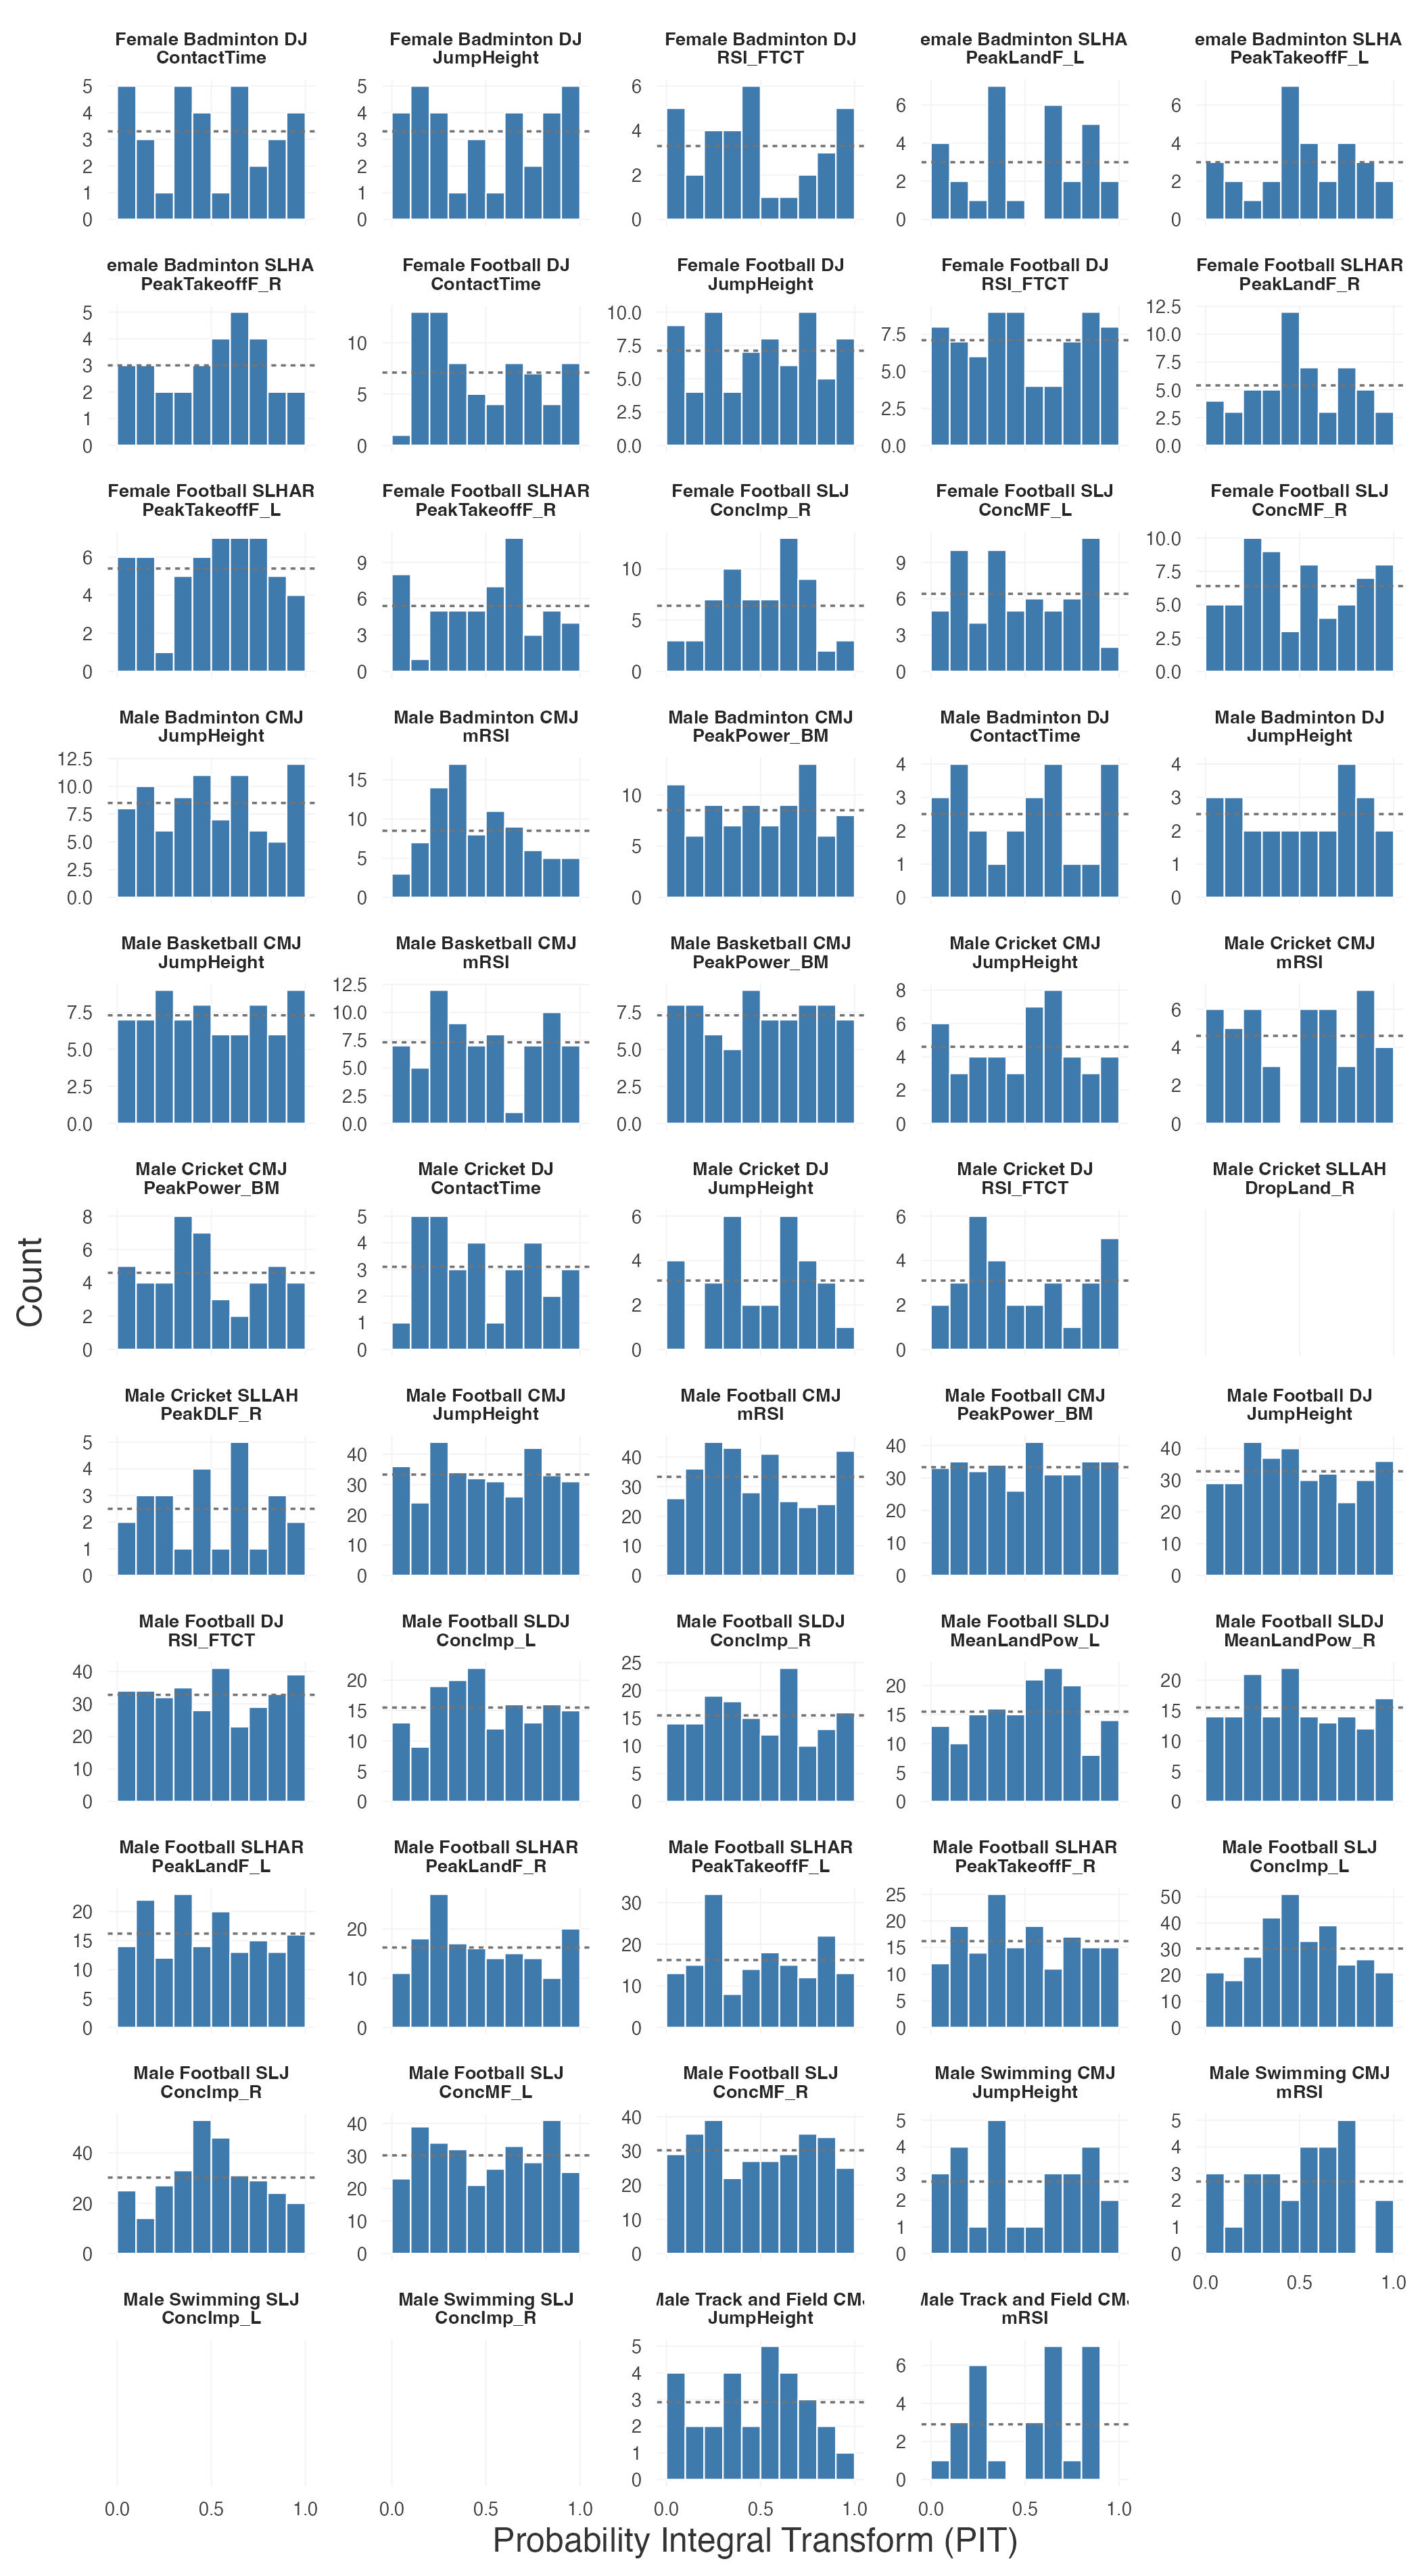
\includegraphics[width=\linewidth]{fig_pit_grid.jpg}
\caption{PIT histograms for every (cohort, metric) pair entering the
joint copula. Dashed grey line: expected count under correct
calibration ($n / 10$ per bin).}
\label{fig:pit_grid}
\end{figure}

\section{Per-cohort CMJ JumpHeight centile bands}
\label{app:centile_bands_grid}
\noindent The age-conditional JumpHeight centile bands
(5/25/50/75/95) from the winning marginal under
Eqs.~\eqref{eq:m1}--\eqref{eq:m3}, one panel per CMJ cohort that
retained JumpHeight at Stage~3. Raw observations are overlaid as light
grey points. The Male Football CMJ panel reproduces the worked-example
band (Fig.~\ref{fig:centiles}, left) so the reader can place that
athlete against the other CMJ cohorts.
\begin{figure}[H]
\centering
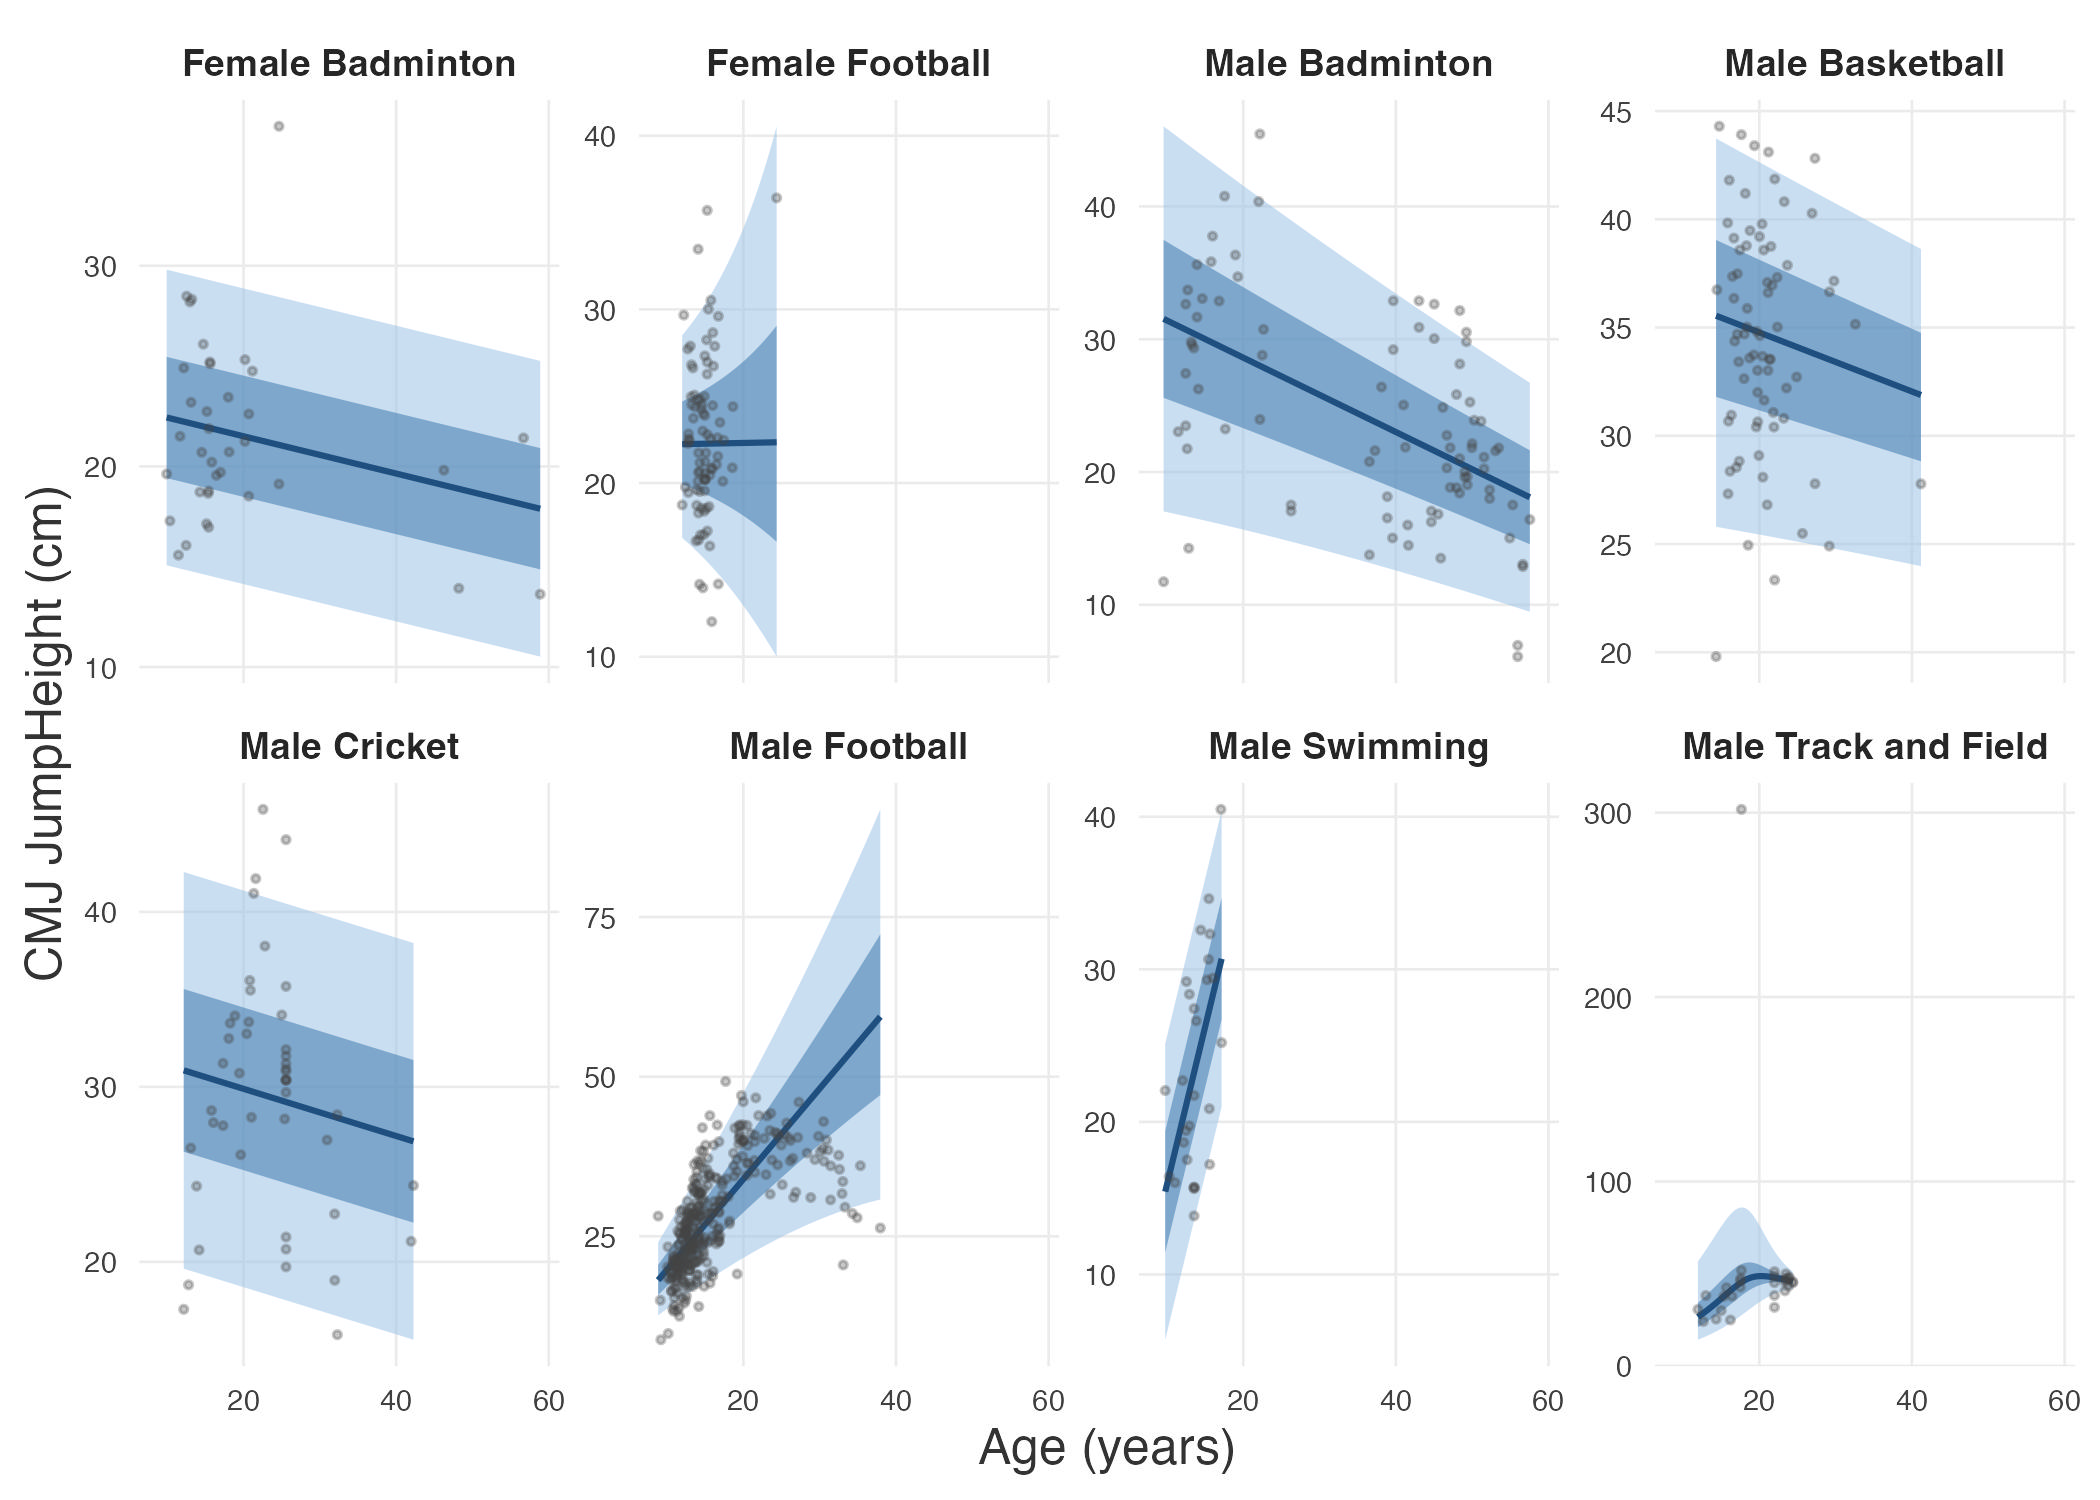
\includegraphics[width=\linewidth]{fig_centile_bands_grid.jpg}
\caption{CMJ JumpHeight centile bands (5/25/50/75/95) per surviving
CMJ cohort. Bands are model-based predictive quantiles at the cohort's
median body mass; raw points overlaid.}
\label{fig:centile_bands_grid}
\end{figure}

\section{Variable-selection sensitivity to the ICC threshold}
\label{app:varsel_sensitivity}
\noindent Stage~3 selection re-run at three ICC$_{(3,1)}$ filter
thresholds (0.4, 0.5 default, 0.7) with the sample-size cap
$n\!\geq\!10\binom{p}{2}$ applied unchanged. The 0.5 column reproduces
body Table~\ref{tab:varsel}; comparing across columns shows which
cohorts gain or lose metrics under stricter or laxer reliability
filtering.
{\footnotesize
\begin{longtable}{lllrp{3.2cm}p{3.2cm}p{3.2cm}}
\caption{\textbf{Sensitivity of variable selection to the ICC$_{(3,1)}$ threshold.} For each cohort, the metrics that would have entered the joint copula at thresholds $0.4$, $0.5$ (default) and $0.7$, after the sample-size cap $n\!\geq\!10\binom{p}{2}$ is applied. The $0.5$ column reproduces Table~\ref{tab:varsel}.}\label{tab:varsel_sensitivity}\\
\toprule
Sex & Sport & Test & $n$ & ICC $\geq 0.4$ & ICC $\geq 0.5$ (default) & ICC $\geq 0.7$ \\
\midrule
\endfirsthead
\multicolumn{7}{l}{\emph{(continued)}} \\
\toprule
Sex & Sport & Test & $n$ & ICC $\geq 0.4$ & ICC $\geq 0.5$ (default) & ICC $\geq 0.7$ \\
\midrule
\endhead
\bottomrule
\endfoot
Female & Badminton & CMJ & 37 & mRSI & mRSI & mRSI \\
Female & Football & CMJ & 82 & JumpHeight, mRSI & mRSI & mRSI \\
Male & Badminton & CMJ & 85 & JumpHeight, PeakPower\_BM, mRSI & JumpHeight, PeakPower\_BM, mRSI & JumpHeight, mRSI \\
Male & Basketball & CMJ & 73 & \emph{none} & \emph{none} & \emph{none} \\
Male & Cricket & CMJ & 46 & JumpHeight, PeakPower\_BM, mRSI & JumpHeight, PeakPower\_BM, mRSI & JumpHeight \\
Male & Football & CMJ & 333 & JumpHeight, PeakPower\_BM, mRSI & JumpHeight, PeakPower\_BM, mRSI & JumpHeight, mRSI \\
Male & Swimming & CMJ & 27 & \emph{none} & \emph{none} & \emph{none} \\
Male & Track and Field & CMJ & 29 & \emph{none} & \emph{none} & \emph{none} \\
\addlinespace[1pt]
Female & Badminton & DJ & 33 & \emph{none} & \emph{none} & \emph{none} \\
Female & Football & DJ & 71 & RSI\_FTCT, ContactTime, JumpHeight & RSI\_FTCT, ContactTime, JumpHeight & RSI\_FTCT, ContactTime, JumpHeight \\
Male & Badminton & DJ & 25 & RSI\_FTCT, ContactTime & RSI\_FTCT, ContactTime & RSI\_FTCT, ContactTime \\
Male & Cricket & DJ & 31 & \emph{none} & \emph{none} & \emph{none} \\
Male & Football & DJ & 328 & RSI\_FTCT, JumpHeight & RSI\_FTCT, JumpHeight & JumpHeight \\
\addlinespace[1pt]
Male & Football & SJ & 188 & ConcMF\_BM & ConcMF\_BM & ConcMF\_BM \\
\addlinespace[1pt]
Female & Football & SLDJ & 55 & MeanLandPow\_R & MeanLandPow\_R & \emph{none} \\
Male & Football & SLDJ & 156 & ConcImp\_R, ConcImp\_L, MeanLandPow\_R, MeanLandPow\_L & ConcImp\_R, ConcImp\_L, MeanLandPow\_R, MeanLandPow\_L & ConcImp\_R, ConcImp\_L, MeanLandPow\_R, MeanLandPow\_L \\
\addlinespace[1pt]
Female & Badminton & SLHAR & 30 & \emph{none} & \emph{none} & \emph{none} \\
Female & Football & SLHAR & 55 & PeakTakeoffF\_R, PeakTakeoffF\_L, PeakLandF\_R & PeakTakeoffF\_R, PeakTakeoffF\_L, PeakLandF\_R & PeakTakeoffF\_R, PeakLandF\_R \\
Male & Football & SLHAR & 166 & PeakTakeoffF\_R, PeakTakeoffF\_L, PeakLandF\_R, PeakLandF\_L & PeakTakeoffF\_R, PeakTakeoffF\_L, PeakLandF\_R, PeakLandF\_L & PeakTakeoffF\_R, PeakTakeoffF\_L, PeakLandF\_R, PeakLandF\_L \\
\addlinespace[1pt]
Female & Football & SLJ & 67 & ConcImp\_R, ConcMF\_R, ConcMF\_L & ConcImp\_R, ConcMF\_R, ConcMF\_L & ConcMF\_R \\
Male & Football & SLJ & 308 & ConcImp\_R, ConcImp\_L, ConcMF\_R, ConcMF\_L & ConcImp\_R, ConcImp\_L, ConcMF\_R, ConcMF\_L & ConcImp\_R, ConcImp\_L, ConcMF\_R, ConcMF\_L \\
Male & Swimming & SLJ & 26 & \emph{none} & \emph{none} & \emph{none} \\
\addlinespace[1pt]
Female & Football & SLLAH & 63 & PeakDLF\_R & PeakDLF\_R & \emph{none} \\
Male & Cricket & SLLAH & 25 & \emph{none} & \emph{none} & \emph{none} \\
Male & Football & SLLAH & 225 & PeakDLF\_R & \emph{none} & \emph{none} \\
\end{longtable}
}


\section{Extended athlete-scoring example}
\label{app:score_extended}
\noindent The same \texttt{score\_athlete()} output as
Table~\ref{tab:score} for five additional, randomly selected athletes
from the worked-example Male Football CMJ cohort. ``Joint pct'' uses
Eq.~\eqref{eq:qjoint}; the 95\,\% bootstrap CI is over $B = 200$
re-samples of the cohort PIT cloud.
\smallskip
\begin{center}
{\small
\begin{tabular}{rrrrrrrrr}
\toprule
Athlete & Age & BM & JH pct & PP$_{\text{BM}}$ pct & mRSI pct & Joint pct & 95\% lo & 95\% hi \\
\midrule
A1 & 13.9 & 50.1 & 53.0 & 40.6 & 47.1 & 97.6 & 95.2 & 99.4 \\
A2 & 10.9 & 38.2 & 43.2 & 13.2 & 26.8 & 42.9 & 27.6 & 52.9 \\
A3 & 26.9 & 73.1 & 14.2 & 23.3 & 35.8 & 75.7 & 67.0 & 83.2 \\
A4 & 18.7 & 63.5 & 69.8 & 75.8 & 63.0 & 89.5 & 81.7 & 93.1 \\
A5 & 13.6 & 49.7 & 98.3 & 96.9 & 48.5 & 34.2 & 25.8 & 45.1 \\
\bottomrule
\end{tabular}
}

\end{center}
\refstepcounter{table}\label{tab:score_extended}

\section*{Acknowledgements}
We thank the coaches and athletes whose performance data
made this work possible, and the Indian Institute of Technology
Bombay for hosting the collaboration.

\section*{Data Availability}
Code, fitted model objects, anonymised per-cohort summaries,
per-athlete score tables (\texttt{verification/results/athlete\_scores\_wide.csv}
and \texttt{athlete\_scores\_long.csv}; one row per athlete-test
occasion with marginal percentiles, joint percentile and 95\,\%
bootstrap interval), and a fully reproducible pipeline are
released at
\url{https://github.com/praveenmaths89/vald-multivariable-centiles}
(a permanent DOI is provided via Zenodo upon acceptance).
The underlying ForceDecks data are held by PhysioQinesis /
Performance Lab in collaboration with IIT Bombay and are
available from the corresponding author upon reasonable request,
subject to the data sharing agreement governing the collaboration.

\section*{Conflicts of Interest}
The authors declare no conflicts of interest.

{\small
\bibliographystyle{plain}
\bibliography{refs}}

\end{document}
